\chapter{Background and Literature Review} \label{chap:background}
% -------------------------
%% QUOTE
\vspace*{\fill}
\epigraph{Those who don't know history are destined to repeat it.}%
{\textsc{Edmund Burke}}
\clearpage{\thispagestyle{empty}\cleardoublepage}
%%
%% Body of the chapter
%%%%%%%%%%%%%%%%%%%%%%
\section{Nanoparticles and Nanomaterials}
If we assumed a range for all the sizes colloids could assume, Nanoparticles \index{nanoparticle} would be at the smaller end of it \citep{Goodwin2009}. The different industries have, in the last decade or two, found significant applications for nanoparticles in manufacturing products with special characteristics. In all these applications, the small size of nanoparticles is exploited for development of new materials, tools and devices. Generally speaking, ``nanoparticles" are particles whose dimensions (at least one dimension) are smaller than 100 nm. At these lengths, special electronic, thermal, mechanical and chemical properties appear (such as greater surface area per volume, higher reactivity with other molecules), the application of which can enable a plethora of new solutions. Figure \ref{cht:NPsurfaceVolume} shows surface area to volume ratio of the same volume of materials in ranges of millimeter, micrometer and nanometer. As illustrated by \citet{Amanullah2009}, conversion of a particle from the millimeter scale to the nanometer scale will multiply its area to volume ratio a million fold. 
\begin{figure}[h]
    \centering
    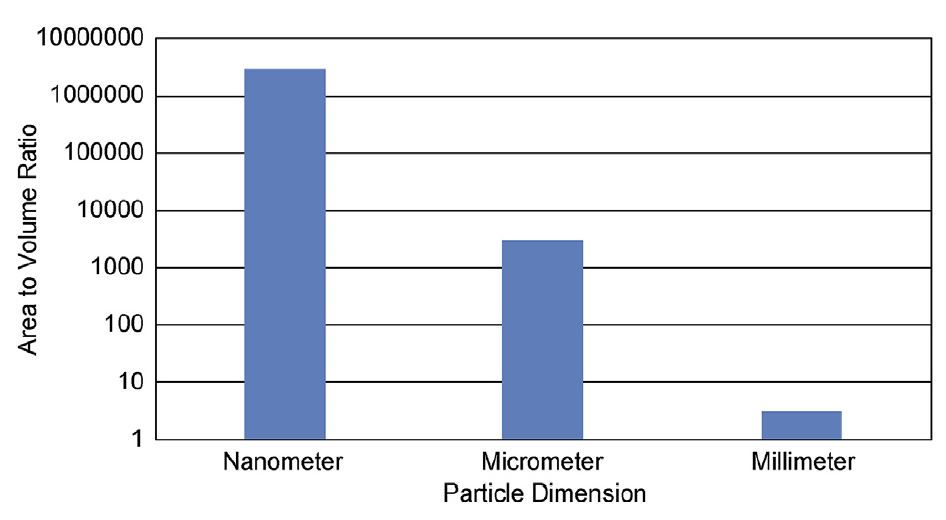
\includegraphics[width=\textwidth]{img/cht/NPsurfaceVolume.png}
    \caption{Surface area to volume ratio of the same volume of materials (adapted from \citet{Amanullah2009})}
    \label{cht:NPsurfaceVolume}
\end{figure}

\citet{Fakoya2017} definet ``Nanomaterials" \index{nanomaterial} as materials that are composed of nanoparticles as part of their structure. Nanomaterials inherit most of the qualities and enhanced properties from the embedded nanoparticles. Compared to regular materials, in nanomaterilas most of the atoms occupy the surface of the particles \citep{Wilson2002}. Nanomaterials are mainly produced by six common methods \citep{Hussainova2010}: electrodeposition \citep{Bera2004}, ball milling \citep{Cao2007}, chemical vapor deposition \citep{AZO2013}, plasma arcing \citep{Shashurin2015}, sol-gel synthesis \citep{Ficai2017}, and the use of natural nanoparticles \citep{Wilson2002}. 

\section{State of the art and applications of nanotechnology in the oil and gas industry}
More recently, the oil industry has started to recognize nanoparticles and nanotechnology as a potential for breakthroughs in all aspects of the industry, from exploration to drilling, from reservoir management to production \citep{Cocuzza2011}. Drilling and completion projects, for example, can benefit from specific characteristics of nanoparticles such as their mechanical strength, corrosion resistance and lightness. The exploration branch can take advantage of nano-sensors for modern monitoring techniques. And of course, reservoir engineers could apply nanotechnology to development of ``smart fluids" for water shut-off and enhanced oil recovery (EOR) \index{EOR} purposes. 

\subsection{Drilling and hydraulic fracturing}
It is interesting to note that naturally occurring nanoparticles have played a role in the oil industry for the past 60 years. An example would be drilling muds \index{drilling mud} which are composed of nanoparticles made of clays (disks of aluminosilicates) which have thicknesses in the range of 1 nm \citep{Krishnamoorti2015} and have significant rheological properties. Still, nanotechnology can play a more promising role in the oil and gas industry by development of synthetic nanoparticles. These types of nanoparticles have carefully controlled functionalities (chemical groups) attached to them, which tailors the chemical interactions, shape and size of the particles to the technical needs of the industry.

Operating conditions, in the recent years, have generally shifted towards harsher and more extreme cases. Deeper reservoirs (sometimes under deepwater environments), horizontal wells and harsh environmental conditions are a few examples. Conventional materials, fluids and cements have only a substandard performance under these conditions. With the advent of nanotechnology, drilling and production operations have benefited from the development of a new group of fluids referred to as \index{smart fluid} ``smart fluids". These fluids improve the performance of said operations by altering wettablity, reducing drag and consolidating formation sand \citep{Wasan2003, Chaudhury2003, Amanullah2009}. Drilling speeds have been improved (at least in the lab scale) by treating the drilling mud with nanoparticles and superfine powders, reducing or even eliminating the damage to the near wellbore formation \citep{Esmaeili2011}.

Drilling fluids carry the cuttings \index{cutting} in the well to the surface, while hydraulic fracturing \index{hydraulic fracturing} fluids transport proppants to the fractured zones around the wellbore. Current fluids used for drilling and fracturing contain particles in the macro and micro range and therefore result in formation damage by leaving thick mud cake around the annulus. According to \citet{Outmans1958}, when there is a pressure difference between the mud column in the borehole and the formation fluid, the drill string sticks to the wall of the wellbore. This effect is referred to as ``differential sticking" and is magnified when low quality drilling muds are used. 

As a result researchers in the drilling area have continuously been looking for better solutions in the development of such fluids, and therefore nanoparticles have started to play a role in recent years. \citet{Amanullah2011} conducted several experiments on water-based muds incorporating nanomaterials. They concluded that using nanotechnology can improve the rheological properties of ``smart" drilling fluids and mitigate the effects of thick and tight mud cakes. 

During drilling operations, there comes a time when it is necessary to change mud types or perform cementing operations. In either case, it would be necessary to separate the old mud from the new mud or the cement. For this purpose, special fluids known as ``spacers" \index{spacer} are used. For example, the residual oil-based muds (OBM) in the wellbore must be removed by the spacer to prevent costly contamination of cement \citep{VanZanten2010}. The rusults from experiments carried out by \citet{Maserati2010} indicated that nano-emulsions (emulsions where: droplet size of internal phase $<$ 500 nm) perform better than common spacers at casing - open hole cleaning and wettability alteration for better adhesion of slurry in the casing - open hole gap. 

Drilling in shale formations \index{shale formation} poses specific challenges to the operator companies. One such challenge is fluid penetration from mud into shale formations which will cause swelling and wellbore instability. In order to solve this problem, the nano-sized pore throats \index{pore throat} of the shale formation must be sealed. However, conventional drilling fluids are made of particles which are too large for this task. Here, nanoparticles can play a role as well. \citet{Sensoy2009} studied four field muds with shales from Atoka and Gulf of Mexico and investigated the effect of addition of silica nanoparticles to the muds. The nanoparticles were able to reduce the permeability of the shale by a factor of 5 to 50, and a as a result, water penetration was reduced by 98\%. Using scanning electron micrographs (SEM) they illustrated the Atoka shale after exposure to nanoparticles. As shown in Figure \ref{fig:npShale} they observed that their nanoparticles could plug small pore throats and in some cases aggregate and seal bigger ones. \citet{Cai2012}, \citet{Riley2012} and \citet{Young2013} performed similar studies for water-based muds, and \citet{Srivatsa2011} for surfactant-polymer based muds using silica nanoparticles and confirmed the reduction in water/filterate invasion observed by \citet{Sensoy2009}.

\begin{figure}[h]
    \centering
    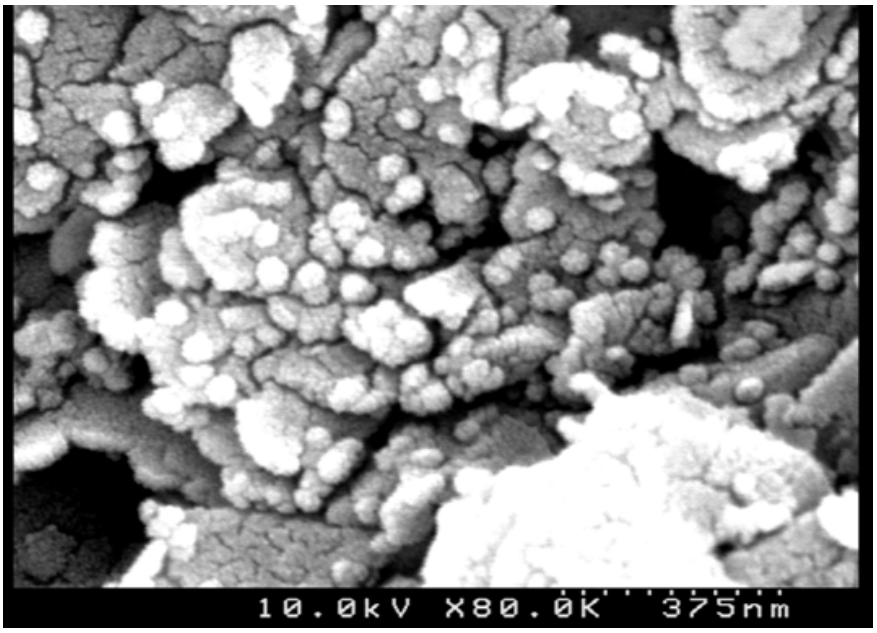
\includegraphics[width=\textwidth]{img/fig/npShale.png}
    \caption{SEM of 20 nm particles within Atoka shale (Dotted scale is 375 nm). source: \citet{Sensoy2009}}
    \label{fig:npShale}
\end{figure}

Research on nanomaterials has also found new solutions in the area of hydraulic fracturing, both for creating viscous fluids and for breaking them down. Fracturing fluids should provide sufficiently high viscosities (in the order of highly viscous gels) for transferring large amounts of proppants and creating fractures \citep{Weaver2002}. \citet{Hurnaus2015} used nanoparticles as crosslinking agents for creating viscous fluids for hydraulic fracturing with lower environmental impact. Meanwhile, \citet{Crews2010} used nanoparticle-associated surfactants in brine to develope a technology for breaking down the residual polymer from hydraulic fractures into easily producible fluids during a post-treatment stage. The resulting Viscoelastic Surfactant fluids (VES) showed crosslinked-polymer-like viscosities. These fluids contained internal breakers that broke the residual polymer without the need to contact reservoir fluids \citep{Crews2007}.

\subsection{Corrosion inhibition}
Corrosion \index{corrosion} costs the oil industry billions of dollars a year by destruction of metallic structures \citep{Brondel1994}, and it only makes sense that modern research has addressed nanomaterials as a potential agent for corrosion inhibition. 

\citet{Jauhari2011} designed a ferrofluid corrosion inhibitor composed of ferromagnetic naonparticles and studied the corrosion behavior of carbon steel in an acidic environment with various concentrations of the nanomagnetic fluid. They observed that increasing the concentration of the nanomagnetic fluid leads to an increase in the inhibition efficiency (up to an optimum concentration) and thus a reduced corrosion rate. 

The experimental resutls of \citet{Murugesan2016} revealed that Nickle based coatings, which are used for inhibiting corrosion, can be improved by the development of metal-matrix-nanocomposite coatings (MMnC). These coatings are synthesized by colliding nanoparticles with the growth surface and encapsulation of these nanoparticles by the depositing Nickle ions. Their nanocomposite coatings were able to outperform the commercially available coatings and therefore extend the lifetime of equipment which are exposed to corrosive and errosive environments. 

\subsection{Logging}
Acquiring subsurface data is inevitable, e.g., during drilling operations or later in the life cycle of a well. Logging operations are those where certain tools are run into the well with the purpose of reading representative, undisturbed and sometimes real time data about reservoir rock and fluid properties. \citet{Singh2006} claimed that an innovative system, which they called \index{nanologging} ``nanologging", could potentially provide more accurate data than logging while drilling (LWD) and measurements while drilling (MWD). In their proposed technique nanorobots are used for the purpose of logging. These robots, which are equipped with the necessary sensors, are circulated into the mud system of the borehole and at the same time they may ``swim" through the mud based on the principle of viscous forces. They would then transmit the acquired real-time data to the surface by means of an electro-magnetic transmitter. 

\subsection{Production}
Migration of formation fines \index{formation fines migration} is a big challenge during production operations. During production from unconsolidated reservoirs, clays and other formation fines migrate towards the production well and cause several problems such as ruining the surface and downhole equipment (in turn causing downtime and replacement costs), permeability reduction and environmental issues \citep{Tiffin1998}. \citet{Huang2008} illustrated the formation fines migration from reservoir to the near-wellbore area into the fracture proppant pack as shown in Figure \ref{fig:fines}. A comparison of Figures \ref{fig:fines1} and \ref{fig:fines2} shows how fines continue to migrate to the pack from all directions and concentrate after a while, forming larger particles and blocking the flow channels near wellbore proppant pack (in this particular case the production drops from 1000 barrels per day (bpd) to 100 bpd in only 3 months. As shown in Figure \ref{fig:fines3} this problem can be remedied by using nanoparticle-treated fracture proppant packs. The high surface enregy of the nanoparticles on the proppants will fixate the fines during production and prevent them from concentration and eventually reduction of oil rates. In recent years, a few research studies have focused on applying nanotechnology to mitigate fine migration effects \citep{Belcher2010,Habibi2011,Ogolo2012,Ahmadi2013}.

\begin{figure}[p] 
    \begin{subfigure}{.8\textwidth}
    \centering
    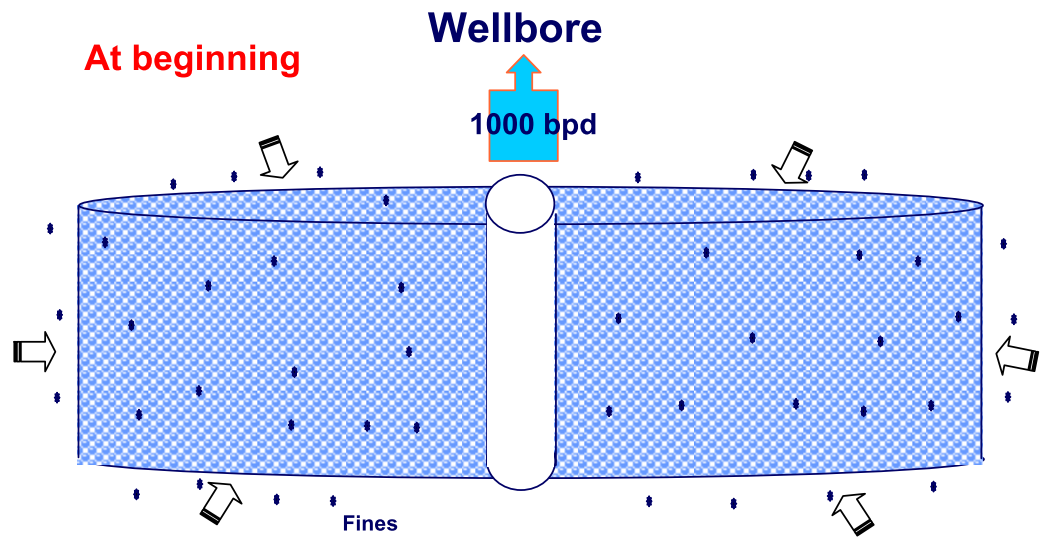
\includegraphics[width=\textwidth]{img/fig/fines1.png}
    \caption{Formation fines carried by formation fluid flow into proppant pack in all directions as well starts producing.}
    \label{fig:fines1}
    \end{subfigure}
    \\
    \begin{subfigure}{.8\textwidth}
    \centering
    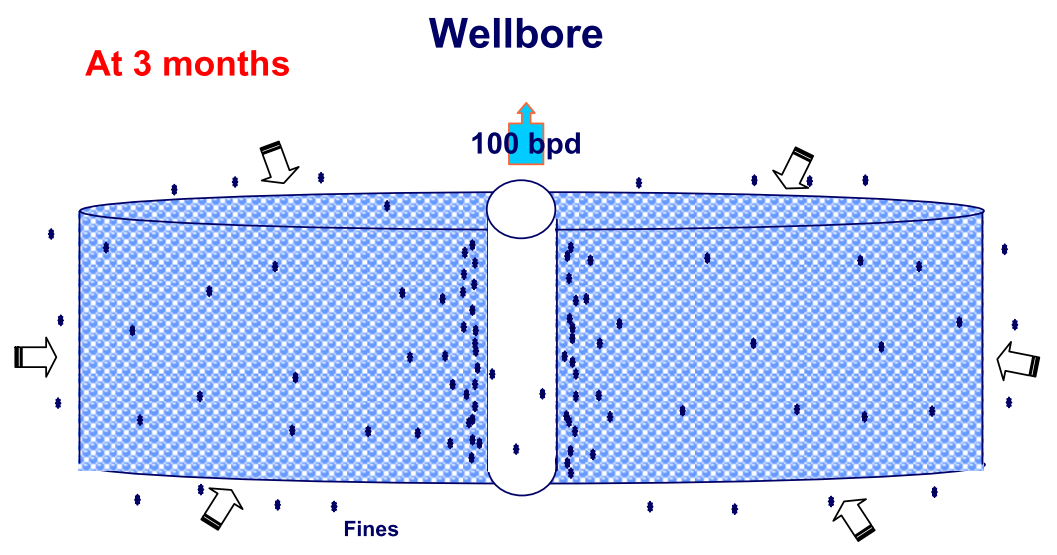
\includegraphics[width=\textwidth]{img/fig/fines2.png}
    \caption{Formation fines migration after several months of well production for non-treated proppant pack.}
    \label{fig:fines2}
    \end{subfigure}
    \\
    \begin{subfigure}{.8\textwidth}
    \centering
    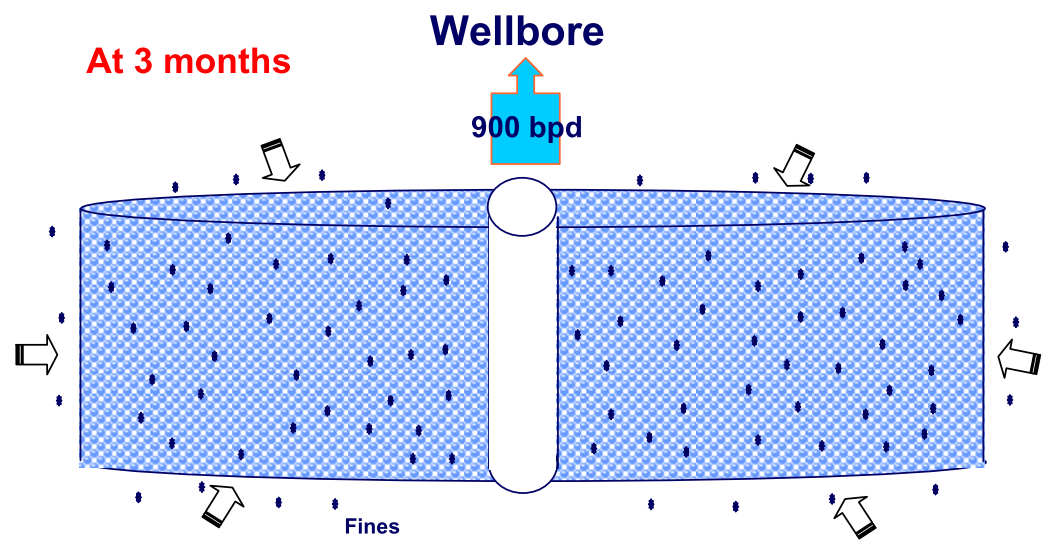
\includegraphics[width=\textwidth]{img/fig/fines3.png}
    \caption{Formation fines fixed in nanoparticle-treated proppant pack.}
    \label{fig:fines3}
    \end{subfigure}
    
    \caption{Formation fines migration. source: \citet{Huang2008}.}
    \label{fig:fines}
\end{figure}

\citet{Ogolo2013} experimentally identified magnesium oxide, aluminum oxide and zinc oxide nanoparticles as candidates for trapping unconsolidated fines. Among the candidates aluminum oxide was had the best performance, while the other two caused some permeability problems. Yet \citet{Huang2015} reported magnesium oxide nanoparticles to be performing well under water injection. They conducted experiments on stabilizing formation clays and fines during water flooding operations using nanoparticles. The results of their experiments indicated that adding 8-nm magnesium oxide particles to injection water would increase sweep efficiency by manipulating local clays and other formation fines and prevent swelling and migration of fines. 

\subsection{Enhanced Oil Recovery}
In order to benefit from nanoparticles for EOR \index{EOR|(} purposes, they first need to be transported and delivered to the desired depths from the injection well within the reservoir. Accordingly, a few studies have addressed transport of nanoparticles through porous media, investigating their stability and breakthrough time in different environments. \citet{Yu2010} investigated transport and retention \index{retention} of aqueous dispersions of paramagnetic iron oxide nanoparticles in sedimentary reservoir rocks. Their coreflood experiments demonstrated that given the right surface coating, high concentrations of paramagnetic nanoparticles can be transported through high and low permeability rocks (Boise sandstone and Texas Cream limestone). 

In another study \citet{Yu2010a} investigated transport of carbon nanoparticles in synthetic sea water (SSW) through dolomite cores from Kuwait and Berea sandstones. The results of this study showed that high ionic strength (1 wt\% KCl) and multivalent ions (\ce{Ca^2+} and \ce{Mg^2+} grew the amount of retention that the nanoparticles experienced, and therefore delayed the breakthrough of nanoparticles dramatically. This underlying theory has been well accepted in the literature: in aqueous suspensions high ionic strength caused by high salt concentration shrinks the electric double layer \index{electric double layer} and reduces the repulsion \citep{Goodwin2009, Tadros2013}. In a later study, \citet{Yu2012}investigated the transport and adsorption of silica nanoparticles in Berea sandstone, Indiana limestone, and dolomite. They observed that nanoparticles could pass through sandstone and limestone without noticeably changing the permeability. However, they could not observe the same effect in dolomite as the cores were plugged and the permeability was reduced. 

Wettability alteration \index{wettability alteration} is one of the major mechanisms exploited by some EOR \index{EOR} methods. To study wettability alteration of water wet rocks obtained from the Niger Delta, \citet{Onyekonwu2010} looked into three types of polysilicon nanoparticles, namely lipophobic and hydrophilic (LHPN), hydrophobic and lipophilic (HLPN) and neutrally wet (NWPN). They reported that NWPN and HLPN dispersed in ethanol successfuly altered wettability and reduced interfacial tension, and recommended them for use in EOR for water-wet formations. \citet{Roustaei2013} evaluated the effect of modified silica nanoparticles on IFT reduction in two different Iranian light and intermediate oil reservoirs. Their results indicated more effective IFT reduction in light oil sandstone reservoirs. 

In another study carried out at NTNU, \citet{Li2013} investigated hydrophilic silica nanoparticles with average single particle size 7 nm through two phase visualization glass micromodel flooding and also core flooding experiments with \index{Berea} Berea sandstones. Their experimental results agreed with earlier research in that silica nanoparticles were successful in reducing IFT between the water and oil phases and making the rock more water wet. As shown in Figure \ref{fig:microGlass}, they illustrated that at high concentrations of nanoparticles, the nanofluids could stabilize the emulsion and break down big oil droplets into smaller ones resulting in improved oil recovery.

\begin{figure}[h]
    \centering
    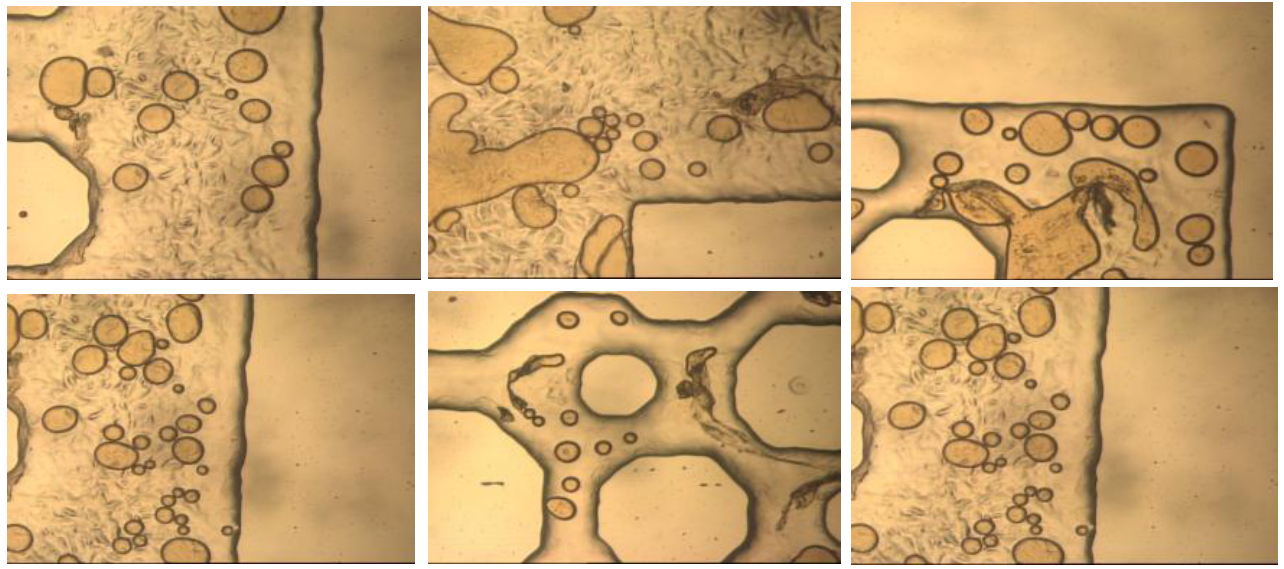
\includegraphics[width=\textwidth]{img/fig/microGlass.png}
    \caption{Visualization glass micromodel experiment with emulsions in higher concentration of nanoparticles. source: \citet{Li2013}}
    \label{fig:microGlass}
\end{figure}

In a later study, \citet{Hendraningrat2014} evaluated how the initial rock wettability would influence the ability of hydrophilic silica-based nanofluids to recover more oil. They used water-, intermediate-, and oil-wet systems with Berea sandstone in a temprature range of 25 - 80~\celsius. Their results showed that the effect of initial wettability was more dominant at higher temperatures. They also reported that using silica nanofluids they could reduce the residual oil saturation, improving oil recovery in all the three wettability cases, although best results were achieved in cased of the intermediate-wet system.   

\citet{Zargartalebi2015} examined whether anionic surfactant flooding would be enhanced in presence of hydrophilic and hydrophobic silica nanoparticles. Their results revealed that additoin of NPs affects the IFT between the oil and the surfactant as a function of NP concentration. The presence of NPs also reduced adsorption of surfactans on the rock surface, and this effect was more dominant with hydrophobic particles. Their subsequent core flooding resulted in improved oil recovery compared to conventional surfactant flooding.

\citet{Ye2013} studided the effect of nanoparticles in \index{polymer flooding} polymer flooding. They synthesized a copolymer by free radical polymerization of acrylamide (AM), acrylic acid (AA), and nano-SiO2 functional monomer (NSFM) as raw materials under mild conditions. Figure \ref{fig:AMAANP} shows the structural difference between the molecular chains of copolymer with and without nanoparticles. As illustrated in Figure \ref{fig:AM-AA-NP}, when nanoparticles were introduced the molecular chains of AM/AA/NSFM consisted of many micro-nano structure units. Their results indicated that this structure had higher apparent viscosity at 500 s$^{-1}$ shear rate, achieved up to 43.7\% viscosity retention rate at 95~\celsius, exhibited higher resistance factor and residual resistance factor resulting in better mobility control and higher oil recovery.
\begin{figure}
    \begin{subfigure}{\textwidth}
    \centering
    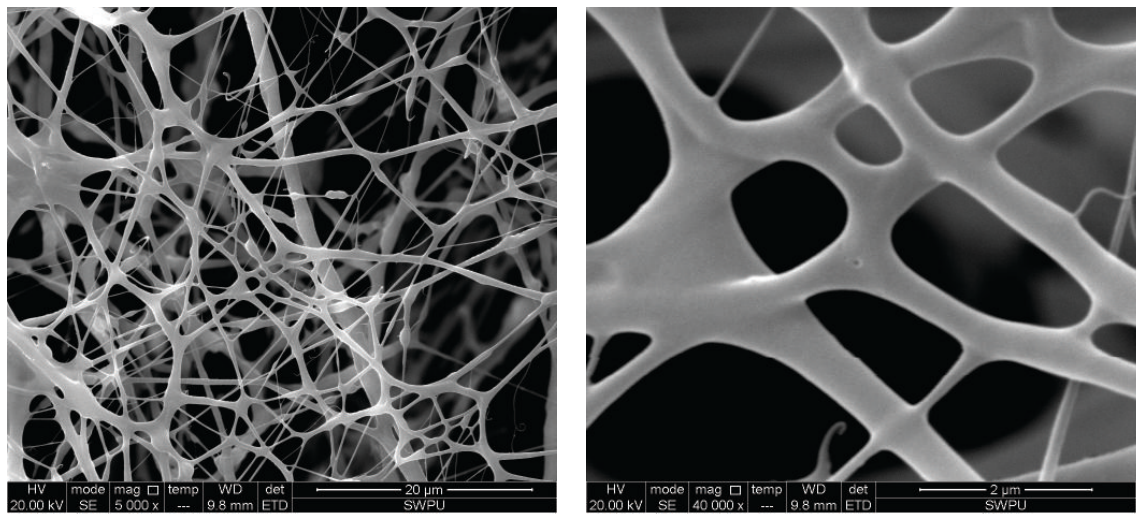
\includegraphics[width=\textwidth]{img/fig/AM-AA.png}
    \caption{SEM images of AM/AA at two magnification scales}
    \label{fig:AM-AA}
    \end{subfigure}
    \\
    \begin{subfigure}{\textwidth}
    \centering
    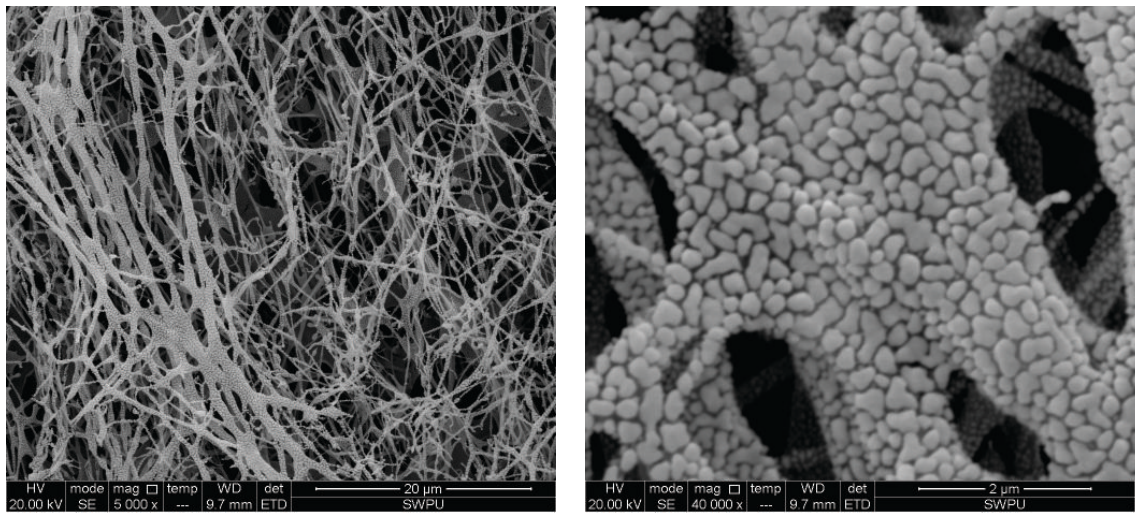
\includegraphics[width=\textwidth]{img/fig/AM-AA-NP.png}
    \caption{SEM images of AM/AA/NSFM at two magnification scales}
    \label{fig:AM-AA-NP}
    \end{subfigure}
    
    \caption{Comparison of the polymer structure of AM/AA with and without NSFM. source: \citet{Ye2013}}
    \label{fig:AMAANP}
\end{figure}    


\ce{CO2} based EOR methods face several challenges. One challenge is early gravity segregation of \ce{CO2} due to lower density compared to water, preventing \ce{CO2} from sweeping lower zones of the reservoir. Another challenge arises due to lower viscosity of \ce{CO2} leading to viscous fingering and early breakthrough of \ce{CO2} through the highly permeable channels in the reservoir. Therefore, in order to reap the benefits of \ce{CO2} injection for EOR, its mobility must be reduced, and the \ce{CO2} foam \index{\ce{CO2} foam} (gas in liquid colloid) must be stabilized. 

Nanoparticles have been the subject of various research studies on the foam stabilization front as well. \citet{Zhang2009} studied the application of nanoparticles in stabilizing foams under high temperature reservoir conditions. \citet{Manan2015} investigated the effects of different types of nanoparticles, namely silicon dioxide, aluminum oxide, copper oxide and titanium dioxide on stabilizing \ce{CO2} foams for mobility control in immiscible gas flooding. They concluded that low concentrations of nanoparticles can bring about high foam resistance and stability, with aluminum oxide particles performing best. \citet{Singh2016} could stabilize foam using surface-modified nanoparticles (SMNPs) both in bulk and porous media. They synthesized SMNPs by partial hydrophobization of alumina-coated silica nanoparticles with a surface modifier. More recently, \citet{Barrabino2018} experimentally compared the effect of graphene oxide, nanographene oxide and partially reduced graphene oxide on stabilizing \ce{CO2} foams. The results of their experiments revealed that nanographene oxide was not suitable for \ce{CO2} EOR purposes due to its hydrophilic nature which results in formation of hydrogels in presence of divalent ions and hinders their transport through porous media.

Some studies such as those carried out by \citet{HamediShokrlu2010, HamediShokrlu2013} have investigated the effect of nanoparticles on EOR methods that address heavy oil production by means of viscosity reduction Fand/or interfacial tension \index{interfacial tension} (IFT) modification. \citet{LI2007} used a nano-nickel catalyst to reduce the viscosity of Liaohe extra-heavy oil by aqua-thermolysis\footnote{\citet{Hyne1986} defines aqua-thermolysis as the interaction of high-pressure/high-temperature water steam with the reactive components of heavy oil and bitumen}. They could successfully upgrade the heavy oil through aqua-thermolysis whereby some of C-S bonds in the extra-heavy oil were broken and the mean molar weight of the heavy oil was reduced. \citet{Alomair2015} reported that right concentration of metal oxide nanoparticles can reduce viscosity and modify IFT for enhanced recovery of heavy oils. Based on their experimental study, silicon oxide (\ce{SiO2}) and aluminum oxide (\ce{Al2O3}) nanofluids yielded superior results than their counterparts, nickle oxide (\ce{NiO}) and titanium oxide (\ce{TiO2}). A mixture of \ce{SiO2}/\ce{Al2O3} with formation water gave the highest oil recovery in their study. They also observed the microscopic structure of said nanoparticles magnified to 25000X with a field emission scanning electron microscope (FESEM), \index{EOR|)} as shown in Figure \ref{fig:npFesem}.


\begin{figure}
    \centering
    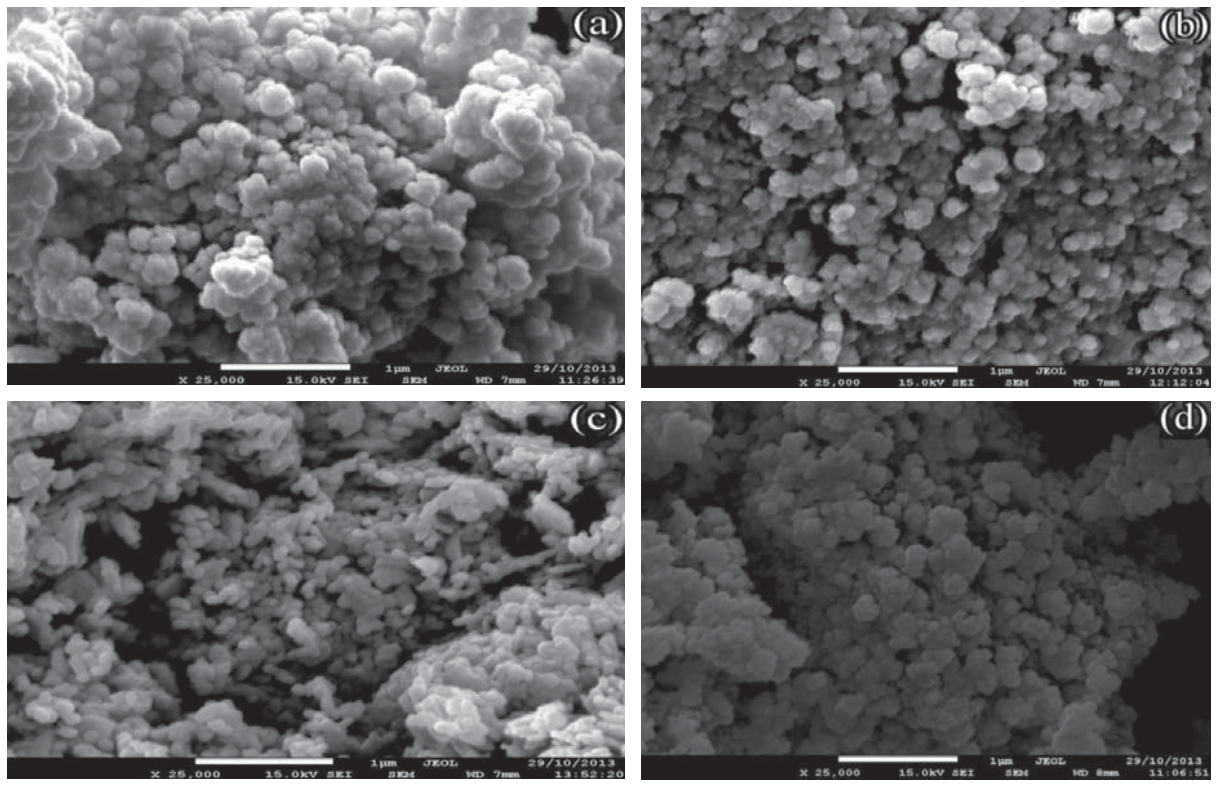
\includegraphics[width=\textwidth]{img/fig/npFesem.png}
    \caption{FESEM images of (a) titanium oxide, (b) aluminum oxide, (c) nickel oxide, and (d) silicon oxide. source: \citet{Alomair2015} }
    \label{fig:npFesem}
\end{figure}



\section{Transport of polymer and nanoparticles in porous media}
The transport of water additives in porous media \index{transport in porous media} is governed by the phenomena \index{retention} retention, adsorption \index{adsorption} and inaccessible pore volume \index{inaccessible pore volume} (IPV) as described by \citep{Lotsch1985}. Changes in composition of the injected solution (e.g., polymer, nanoparticles, salt concentration) affect the responses measured by various sensors. Figure 5.1 shows a few idealized cases of such responses. An ideal piston-like plug flow would look like a step function. However, the real-world effect from dispersion reforms the step function into a curve.

Inaccessible pore volume and retention can shift the curve in Figure \ref{fig:ipvRet1}. The portion of the porous media that cannot be accessed by the particle under study (e.g., the polymer) is referred to as inaccessible pore volume (IPV). The reduced accessible pore volume results in a faster transport of the particles across the porous medium and therefore shifts the response curve to the left. On the other hand, some of the particles under study can be adsorbed on the surface of the rock (adsorption) or are stuck and filtered in small pore throats \index{pore throats}\index{mechanical entrapment} (mechanical entrapment). These effects delay particle flow through porous media, which are collectively referred to as \index{retention} retention. As a result, the response curve is shifted to the right. 

One should only expect the effect of dispersion on responses for step changes in the salt concentration. However, polymer and nanoparticle responses can experience any combination of effects from dispersion, IPV, retention, and flooding history.

\begin{figure}[h!]
    \centering
    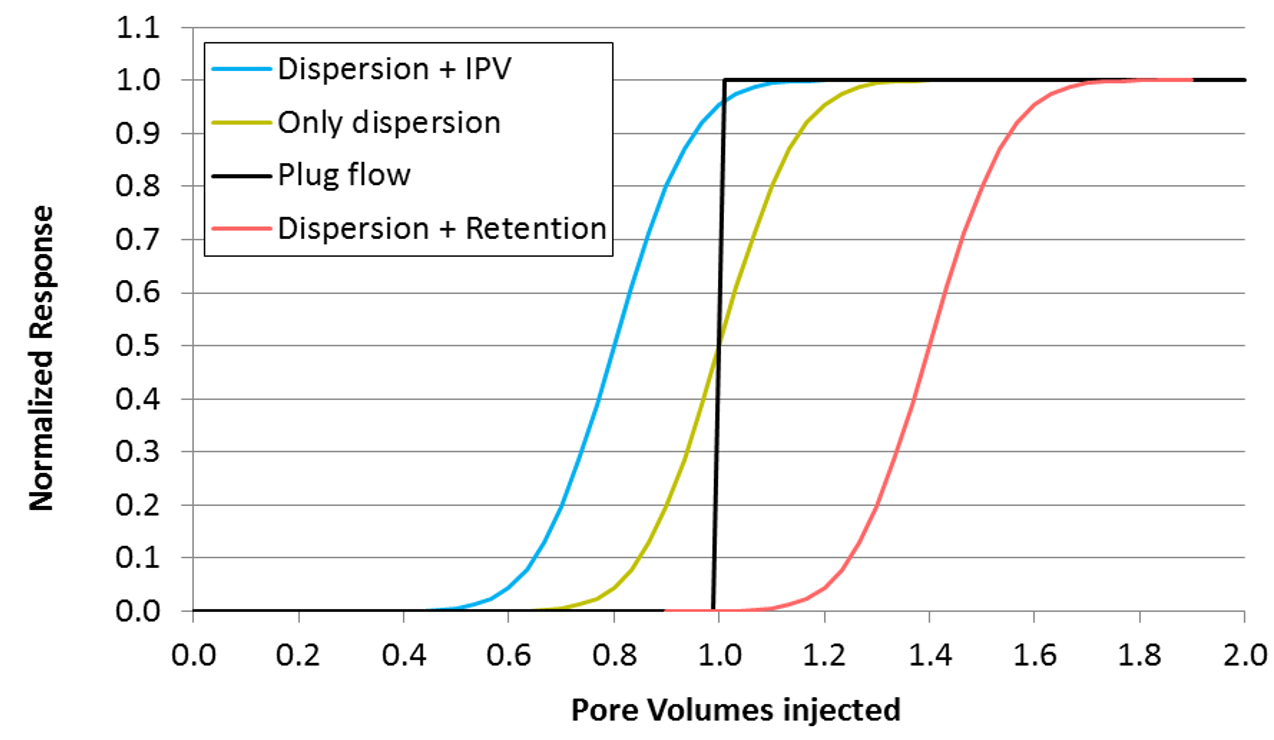
\includegraphics[width=\textwidth]{img/fig/ipvRet1.png}
    \caption{Effect of dispersion, inaccessible pore volume (IPV) and retention on relative responses.}
    \label{fig:ipvRet1} % 5.1
\end{figure}

In order to determine inaccessible pore volume \index{inaccessible pore volume} of e.g., polymer, one can compare the production profiles of polymer and a tracer as a function of pore volumes injected. Figure \ref{fig:ipvRet2} illustrates such a comparison. The relative response of polymer is the ratio of measured effluent concentration to the injected concentration. The tracer should ideally have no IPV, i.e., the area below the tracer response should be equal to one. Changing the concentration in salt tracer will yield a close enough response. The area between the two responses determines the IPV.

\begin{figure}[h!]
    \centering
    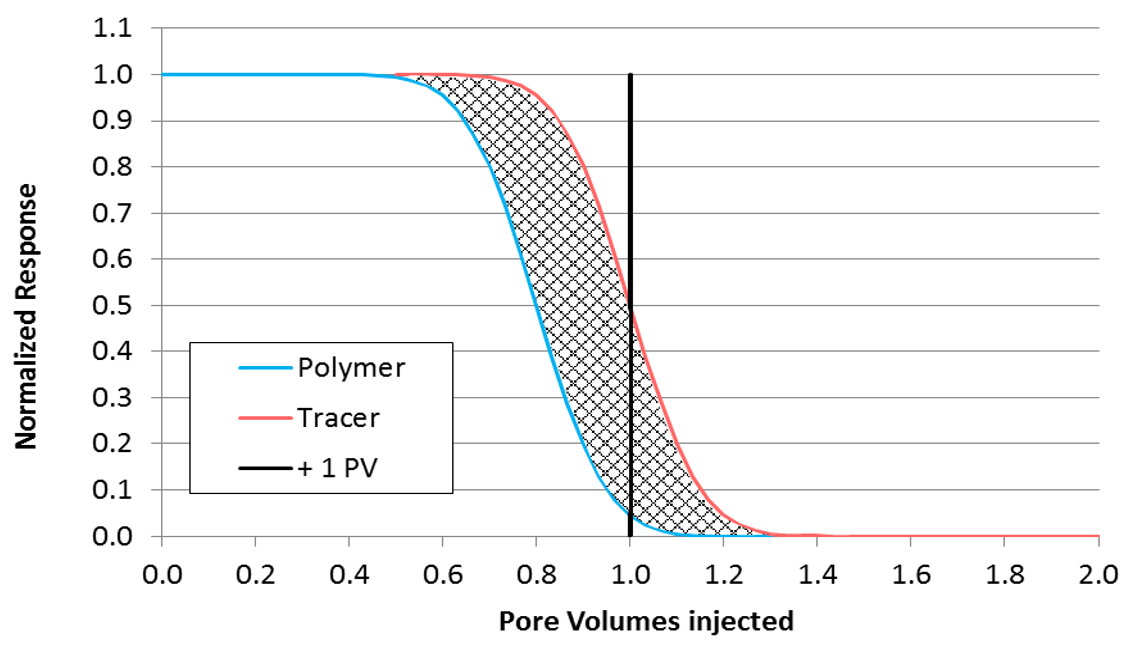
\includegraphics[width=\textwidth]{img/fig/ipvRet2.png}
    \caption{Responses after changing the injected solution from a polymer solution to a solution containing only a tracer ion at a different concentration. The difference in areas defines the inaccessible pore volume.}
    \label{fig:ipvRet2} % 5.2
\end{figure}

Provided that the adsorption of polymer is irreversible and no mechanically entrapped polymer is released during water injection, the IPV will result in a response curve with an area under the curve of less than 1. Thus, IPV for polymer will be a positive value. However, if the system experiences desorption of the mechanically entrapped component, the area under the curve may become larger than the tracer area, resulting in a negative IPV indicating release of retained component. 

Total retention of a component in the rock depends on adsorption and mechanical entrapment. A multi-slug experiment can be used to quantify adsorption. Assuming that adsorption for the component under study were irreversible, all the adsorption happened in the first slug, i.e., no more adsorption took place during the second slug, and the magnitude of mechanical entrapment in both slugs were equal, one can compare the relative responses from the two slugs to find adsorption for the component. This is illustrated in Figure \ref{fig:ipvRet3}.

\begin{figure}[h!]
    \centering
    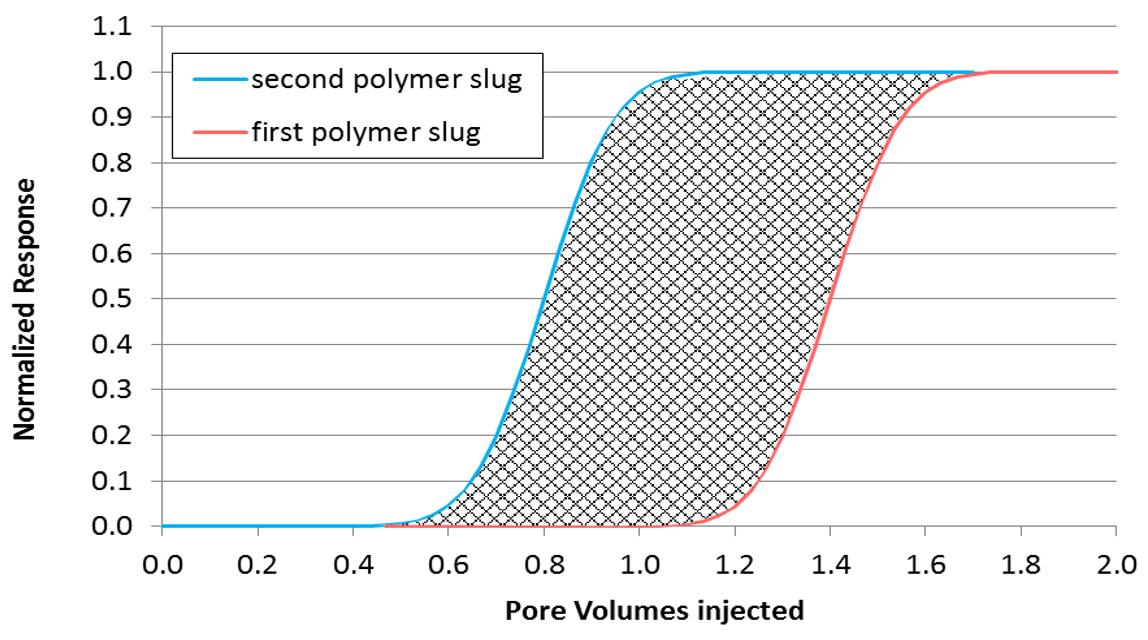
\includegraphics[width=\textwidth]{img/fig/ipvRet3.png}
    \caption{Effect of dispersion, inaccessible pore volume (IPV) and retention on relative responses.}
    \label{fig:ipvRet3} % 5.3
\end{figure}


\section{Overview and properties of gel systems}

A \index{gel} gel system, as referred to in this work, is a polymer solution that has gone through gelation to form a highly viscous and immobile material in the porous formation. The properties of gels in terms of their basic chemistry are discussed in this section, and general overview about polymers is introduced.

\index{polymer} Polymer, as a word consists of two parts: “poly” (many) and “mer” (parts) . A polymer is a macro-molecule that is made of repetitive smaller molecules, referred to as monomers, which are either covalently or ionically bonded. Despite the simple concept of polymers, it was not accepted until late 1930’s, as Hermann Staudinger laboratory results were successful in synthesizing polymers, and obtained because of it the Noble Prize in Chemistry in 1953 \citep{Roberts1977}.

Polymers have different physical and mechanical properties compared to their original
monomers. This is due to the significant difference in the length to diameter ratio between the polymer and its original monomer constituents \citep{Ghosh2006}. Figure \ref{fig:polymer} shows a polymer molecule composed of small monomers.

\begin{figure}
    \centering
    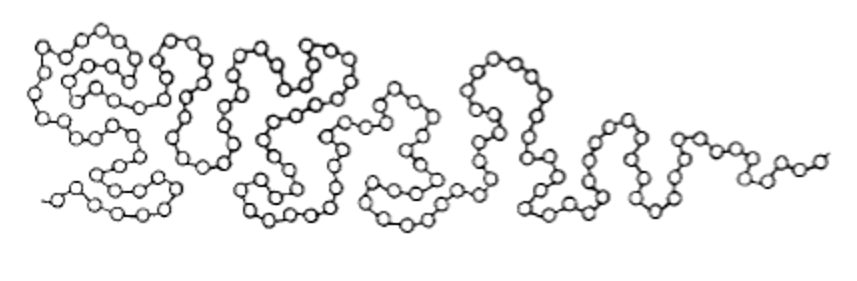
\includegraphics[width=\textwidth]{img/fig/polymer.png}
    \caption{Polymer consisting of several attached monomers (circles) \citep{Ghosh2006}}
    \label{fig:polymer} % 2.1
\end{figure}

Figure \ref{fig:polymonomer} shows a synthetic polymer, referred to as polyacrylamide (PAM) which is one of the most applied polymers in conformance enhancement operations due to its low cost and its good viscosifying properties \citep{Kabir2001}. The monomer (left) can be repeated multiple times in the sequence of the polymer (right) to obtain the desired properties.

\begin{figure}
    \centering
    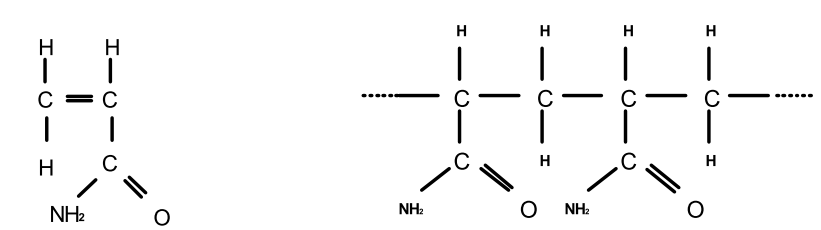
\includegraphics[width=\textwidth]{img/fig/polymonomer.png}
    \caption{Monomer: Amide (left) and polymer: polyacrylamide (right) \citep{Kabir2001}}
    \label{fig:polymonomer} % 2.2
\end{figure}

\subsection{Gel system types}

Gels can be divided into organic and inorganic. Inorganic gels include silicate-based, and Al(III)-based. Organic polymers can be classified in different ways, e.g. based on their origin, thermal response, mode of formation, line structure, physical properties, tacticity, and crystallinity \citep{Ghosh2006}. In the petroleum industry, organic polymers are often classified based on their origin. This includes natural polymers, i.e. biopolymers such as Xanthan and Scleroglucan \citep{Al-Muntasheri2012}, and synthetic polymers such as polyacrylamides, which are usually used in their partially hydrolyzed form, hereafter called \index{partially hydrolyzed polyacrylamide} HPAM \citep{Finch1992}. This report only addresses organic gel systems.

Polyacrylamide-based polymers have been used largely in water diversion operations throughout the history of the petroleum industry due to their low cost comparted with other gel-systems, and due to the good mechanical strength of the formed gel. 

\subsection{Polyacrylamide based gels \label{sec:PolyacrylamideGels}} 
Throughout the history of the petroleum industry, polyacrylamide-based gels were most commonly used in water diversion operations \citep{Al-Muntasheri2005, Ball1984} (Al-Muntasheri et al. 2005; Ball and Pitts 1984). In chemistry, acrylamide can be referred to as acrylic amide. Figure \ref{fig:acrylamide} shows the chemical formula of acrylamide (right) and the acryloyl group (left). The symbol “R” in the figure represents the possibility of having different group of atoms; in which the presence of \ce{NH2} makes the chemical structure defined as acrylamide.

\begin{figure}
    \centering
    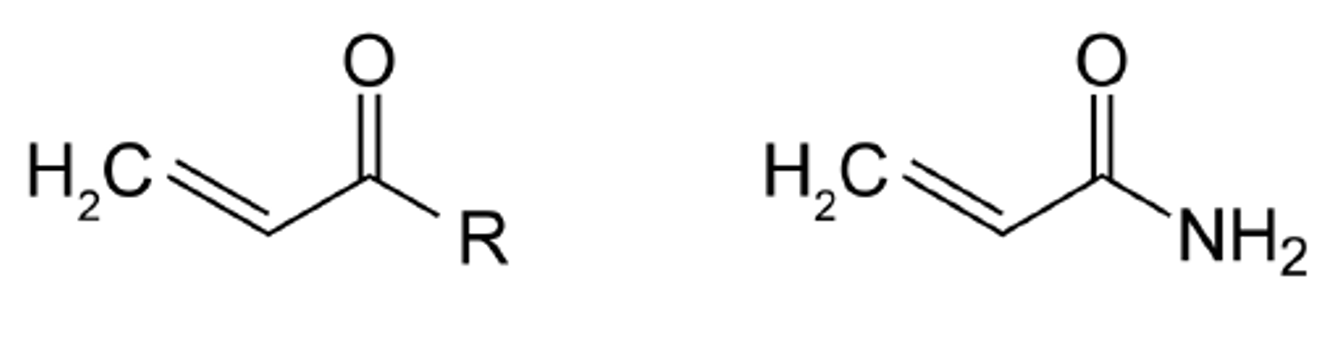
\includegraphics[width=\textwidth]{img/fig/acrylamide.png}
    \caption{Acryloyl group (left) and acrylamide (right)}
    \label{fig:acrylamide} % 2.3
\end{figure}

PAM-solutions undergo hydrolysis, i.e., the reaction of the amide groups of the acrylamide solution with alkaline solutions resulting in carboxylate groups and ammonia. Hydrolysis of acrylamide is shown in Figure \ref{fig:amideHydrol}. The result is a partially hydrolyzed polyacrylamide, \index{partially hydrolyzed polyacrylamide} HPAM. The degree of hydrolysis, $\tau$ , can be defined as:

\begin{equation}
    \tau = \frac{y}{x+y}
\end{equation}							

where $y$ is the molar concentration of the yielded carboxylate groups and $x$ is the molar concentration of the amide groups \citep{Al-Muntasheri2012}.

\begin{figure}
    \centering
    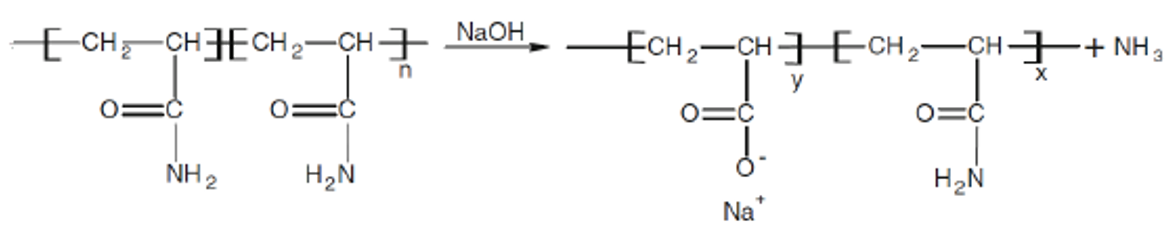
\includegraphics[width=\textwidth]{img/fig/amideHydrol.png}
    \caption{Hydrolysis of amide groups at high pH conditions \citep{Al-muntasheri2008}}
    \label{fig:amideHydrol} % 2.4
\end{figure}

Partially hydrolyzation of PAM is important as the negatively charged carboxylate groups are needed to initiate the gelation process in the presence of organic or inorganic cross-linkers. Al-Muntasheri, suggests that there must be at least 1 mol of carboxylate groups before crosslinking can take place. However, there exists an upper limit for hydrolysis that if it is exceeded, the formed gel might either get weaker or precipitate \citep{Al-Muntasheri2007}. When crosslinking is taking place, i.e. the gelation process has been initiated, there exists a threshold value at which the viscoelastic properties dominate the mechanical properties of the polymer solution. At this stage, which is referred to as the sol-gel transition period, the solution is better described as a gel \citep{Albonico1994}.

HPAM requires a cross-linker \index{cross-linker} to undergo gelation. Normally, the gelation time can take several hours, i.e. the time for the gellant (polymer in aqueous state) to become a gel. \cite{Sydansk1993} Sydansk (1993) described a method in the literature to identify the gradual changes observed in the gellant until it becomes a gel, based on its physical behaviour.

These cross-linkers can be either organic or inorganic \citep{Al-Muntasheri2012}. The selection of either type is dependent on the specific type of application and reservoir conditions \citep{Ball1984}. The amount of the added crosslinker to the aqueous solution plays an important role as low amounts of it may result in long term stability issues, and high amounts arise the probability of having syneresis \citep{Sydansk1993, eggert1992}. Syneresis imposes a significant issue as the volume of the formed gel is reduced, secondary channel paths are created, resulting in a failure of the water-diversion application \citep{Al-Muntasheri2007}. However, in general, it has been observed that higher concentrations of cross-linkers result in more viscous gels as shown in Figure \ref{fig:crosslinkerConc}, given that the level of exceeding syneresis threshold is not reached.

\begin{figure}
    \centering
    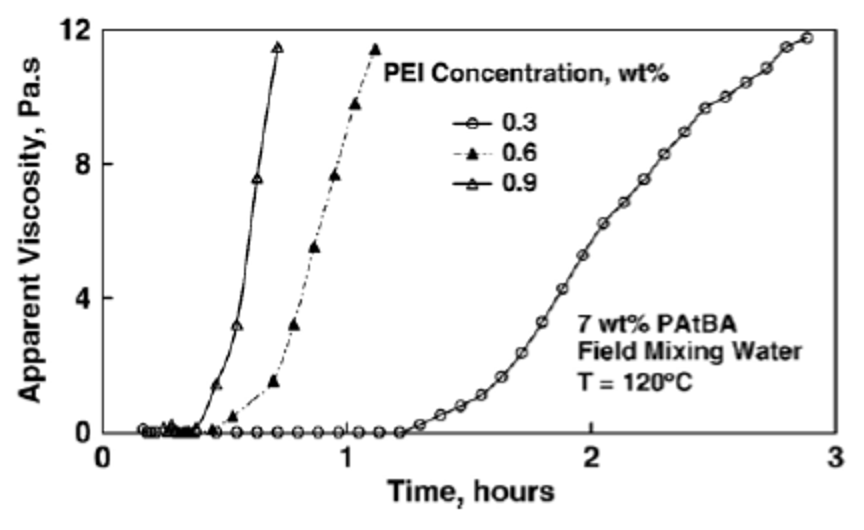
\includegraphics[width=\textwidth]{img/fig/crosslinkerConc.png}
    \caption{Effect of increasing crosslinker (polyetheyleneimine, PEI) concentration on viscosity vs. time \citep{Al-Muntasheri2007}}
    \label{fig:crosslinkerConc} % 2.5
\end{figure}

Inorganic cross-linkers are often referred to as metal crosslinking agents. As the negatively charged (anions) carboxylate groups will chemically bond with the positively charged (cations) cross-linkers, the aforementioned gelation procedure will be initiated. This type of bonding, i.e., ionic bonding, is relatively a weaker type of bonding, as it precipitates at temperatures higher than 75~\celsius, compared with the covalent bond, formed in organic cross-linkers \citep{Al-Muntasheri2005}. Inorganic cross linkers include \ce{Al^3+}, \ce{Zr^4+}, \ce{Cr^3+}, where the latter is the most common cross-linker. Furthermore, \ce{Cr^3+} has the possibility to crosslink biopolymers such as Xanthan which is expensive and difficult to be implemented in large-scale water diversion projects \citep{Al-Muntasheri2012}. However, the application of \ce{Cr^3+} in several countries is limited due to environmental concerns. This will be discussed more in Section \ref{sec:environmental}.

Organic cross linkers were introduced in the industry in order to overcome the limitation of temperature ranges\citep{Al-Muntasheri2005}. As previously mentioned, covalent bonds are much more stable compared to ionic bonds. Examples of organic cross linkers include aldehydes, phenol-formaldehyde and polyetheyleneimine. The polyacrylamide-phenol/formaldehyde system is a good example on an organically cross-linked gel, and has been reported to withstand the temperature of 121~\celsius~ for about 13 years. However, the use of this gel has been limited due to environmental concerns.

\section{Gel systems behaviour in porous media}

Several gel-systems have different chemical, and physical properties that are needed in the water-diversion applications. Basically, for in-depth water-diversion programs, it is appreciated to use a gel that blocks the high-permeable formation, flows easily through the porous rock before gelation takes place, forms an in-situ highly viscous material that dramatically minimizes the permeability, and shows minimal degradation signs when aged for several years. Retention, deposition, and adsorption are some of the critical parameters that affect the application of a particular gel-system. In this section, the aforementioned properties are discussed.

\subsection{Particle transport and deposition in porous media} \index{transport in porous media} The behavior of the small-sized particles, e.g., the size of silicate particles to be injected in the reservoir, can be modeled using the classical fine particle transport \citep{Stavland2011}. They discussed several models regarding particle deposition such as Gruesbeck and Collins (1982), Bedrikovetsky et al. (2010), and Guedes et al. (2009). Figure \ref{fig:finesDeposition} shows the deposition of fine particles along the core length (x) using Gruesbeck and Collins simple model. The relative fines concentration, $c/c_0$, can be described as follows:

\begin{equation}
    \frac{c}{c_0} = e^{\frac{-\phi bx}{u}}
\end{equation}

where $\phi$ is the porosity, $b$ is a constant independent of the flowrate, $x$ is the distance, and $u$ is the flowrate. The values used in Figure \ref{fig:finesDeposition} are $\phi = 0.22$ and $b = 1*10^{-5}$ m/s \citep{Stavland2011}. The flowrate is varied as shown in Figure \ref{fig:finesDeposition}, and indicates that at low velocities, higher deposition of particles takes place.

\begin{figure}
    \centering
    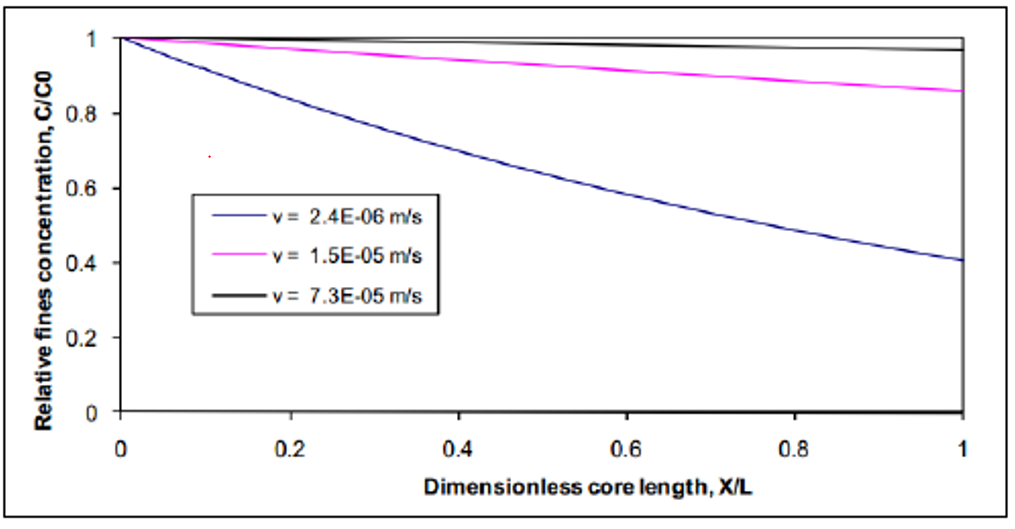
\includegraphics[width=\textwidth]{img/fig/finesDeposition.png}
    \caption{Deposition of fines along the core length \citep{Stavland2011}}
    \label{fig:finesDeposition} % 2.6
\end{figure}

Retention \index{retention} can occur in two different ways, by rock adsorption \index{adsorption} of the injected polymer solution and possibly also by mechanical entrapment \index{mechanical entrapment} as shown in Figure \ref{fig:retention} \citep{Nabzar1996}. At high velocities, no bridging takes places which is likely due to the high viscous forces \citep{Stavland2011}. As the velocity is decreased, bridging is initiated. Eventually, accumulation takes place, and the pore throat becomes plugged. In the literature, several authors reported laboratory experiments for gel system solutions where effect of wettability, mobility reduction, and polymer injection flowrate on retention were examined\citep{Broseta1995, Cohen1986, Idahosa2016}.

\begin{figure}
    \centering
    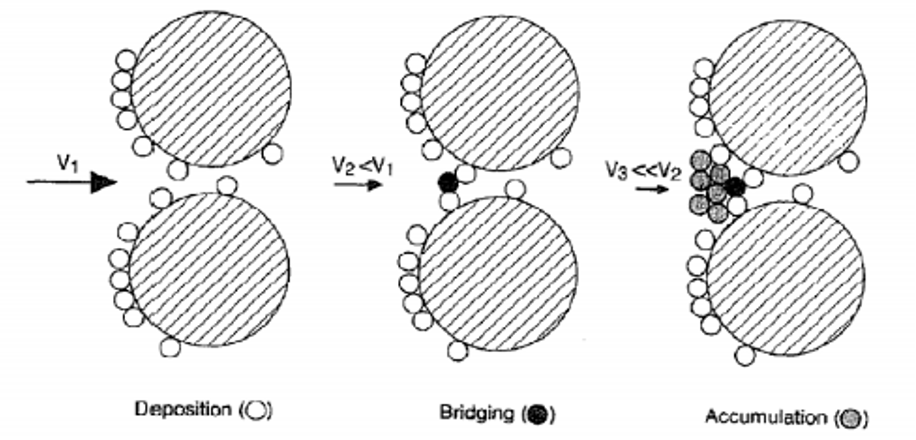
\includegraphics[width=\textwidth]{img/fig/retention.png}
    \caption{Steps of retention at the grain/pore level \citep{Nabzar1996}}
    \label{fig:retention} % 2.7
\end{figure}



\section{Gel systems properties and effects}
There exist several factors that can alter the gelation time, the viscosity as well as the stability of the formed gel-system. These factors include temperature, salinity, pH, and the formation hardness. The main motivation for understanding these effects is to design and select a proper gel-system that is compatible with the reservoir conditions. This section is dedicated solely for polyacrylamide-based polymers properties and effects.

\subsection{Temperature effects} \label{sec:tempEffects}

Reservoir temperature is a major factor that influences the selection criteria of the gel-system to be used in the design of water conformance programs. As discussed earlier, for in-depth water diversion applications, gelation time should be of several weeks, its magnitude depending on characteristics of the reservoir and the nature of the job from an operational standpoint. One of the challenges encountered using \ce{Cr^3+}/HPAM-based \index{partially hydrolyzed polyacrylamide} polymers is the short gelation times above 60~\celsius~ \citep{Albonico1994}. The use of such gel systems is possible for near wellbore treatments at low temperature conditions. However, if the temperature is slightly elevated, other considerations should be taken such as the use of un-hydrolyzed PAM and pre-cooling of the near wellbore region \citep{Albonico1994,Al-Muntasheri2012}. Table \ref{tab:gelTimevTemp} shows the gelation times vs temperature for \ce{Cr(acetate)3}/PAM gels.

\begin{table} 
\centering
\caption{Gelation times vs temperature for \ce{Cr(acetate)3}/HPAM gels \citep{Albonico1994}}
\label{tab:gelTimevTemp} % 2.1
\begin{tabular}{c c } 
\toprule
\textbf{Temperature} & \textbf{Gelation time}\\
~[\celsius] & [hour]\\
\midrule 
60   & 48\\
90   & 2\\ 
120   & $<0.1$\\ 

\bottomrule
\end{tabular}
\end{table}

Albonico et al., proposed the use of gelation-retarding additives in order to reach temperatures at the range of 150~\celsius. \ce{Cr^3+}/HPAM reacts to form a gel very fast as the temperature increases, which makes it not very useful in water-diversion applications. Several complexing agents have the ability to retard the gelation by capturing \ce{Cr^3+} \index{\ce{Cr^3+}} ions in form of complexes that are not reactive with the polymer. However, after a certain period of time, \ce{Cr^3+} ions are released and the gelation is initiated. The rate at which \ce{Cr^3+} is released from the complexes is dependent on the complexing agent. Table \ref{tab:gelTimeHpam} shows gelation times of HPAM solutions with Cr3+ complexes at 90~\celsius. 

\begin{table} 
\centering
\caption{Gelation times of HPAM solutions with \ce{Cr^3+} complexes at 90~\celsius \citep{Albonico1994}}
\label{tab:gelTimeHpam} % 2.2
\begin{tabular}{l c } 
\toprule
\textbf{Cr(III) complex} & \textbf{Gelation time}\\
 & [hour]\\
\midrule 
\ce{Cr(NO3)3}  &                $< 0.02$    \\
\ce{Cr(acetate)3}  &            $< 0.12$    \\ 
\ce{K2Cr(glycolate)3}  &        1           \\ 
\ce{Cr(salicrylate)3}  &        1           \\
\ce{Cr(bipyridine)3(ClO4)3}  &  8           \\
\ce{Na3Cr(malonate)3}  &        48          \\

\bottomrule
\end{tabular}
\end{table}

In addition, it has been proven experimentally that extended delays can be obtained by adding non-complexing agents. A linear relationship between the gelling time and concentration has been found. 

Table \ref{tab:gelRetardAgent} presents the results obtained by Albonico et al. showing that the concentration of the non-complexing retarding ligands can significantly enhance the gelation time. However, it is important to note that adding excessive amounts of retarding ligands has an opposite effect as it can block and disable the initiation of gelation. This is because the \ce{Cr^3+}/ligand complexes become more stable compared to the Cr3+/polymer complexes. Therefore, extensive laboratory trials should be conducted before considering field-scale applications \citep{Albonico1994}.


\begin{table} 
\centering
\caption{Observed range of gelation times of \ce{Cr(malonate)3}/PAM-AMPS in SSW with different retarding agents \citep{Albonico1994}}
\label{tab:gelRetardAgent}  % 2.3
\begin{tabular}{l c c } 
\toprule

\multirow{2}{9em}{\textbf{Retarding Ligand}} & \multicolumn{2}{c}{\textbf{Gelation time (hours)}}\\
\cmidrule{2-3}
 & 90~\celsius & 120~\celsius\\
\midrule 
Gycolate      & 0.9 - 59  &     0.25 – 17      \\
Salicylate    & 0.9 - 27  &     0.25 – 17       \\ 
Malonate      & 0.9 - 215  &    0.25 - 42    \\ 

\bottomrule
\end{tabular}
\end{table}

\citet{Sydansk1993} reported as well that it is possible to obtain gels that can be applied to high temperature reservoirs reaching 126~\celsius using \ce{Cr^3+}-carboxylate complex with low molecular weight and HPAM with a low degree with hydrolysis. The carboxylate anion suggested by Sydansk is ``\textit{acetate}" its availability and low price as a commodity. Moreover, it is important to note that Sydansk’s experiments were based on near-wellbore treatments. 

According to Sydansk, for intermediate reservoir temperatures of about 60~\celsius, low HPAM concentration (1 wt. \%) restricted the formation of the gel. In addition, at low hydrolysis levels ($<0.1$), gelation was not observed. Concentrations of 2, 3, and 4 wt. \% were investigated in the experiments and showed formation of rigid gel according to the experiment specifications. The polymer had a molecular weight of 2 MDa, the degree of hydrolysis was 0.9 and the temperatures was 60~\celsius~ or less. The cross-liker was \ce{Cr(acetate)3}. Figure \ref{fig:viscSydansk} shows the development of the viscosity with time for different HPAM concentrations.

\begin{figure}
    \centering
    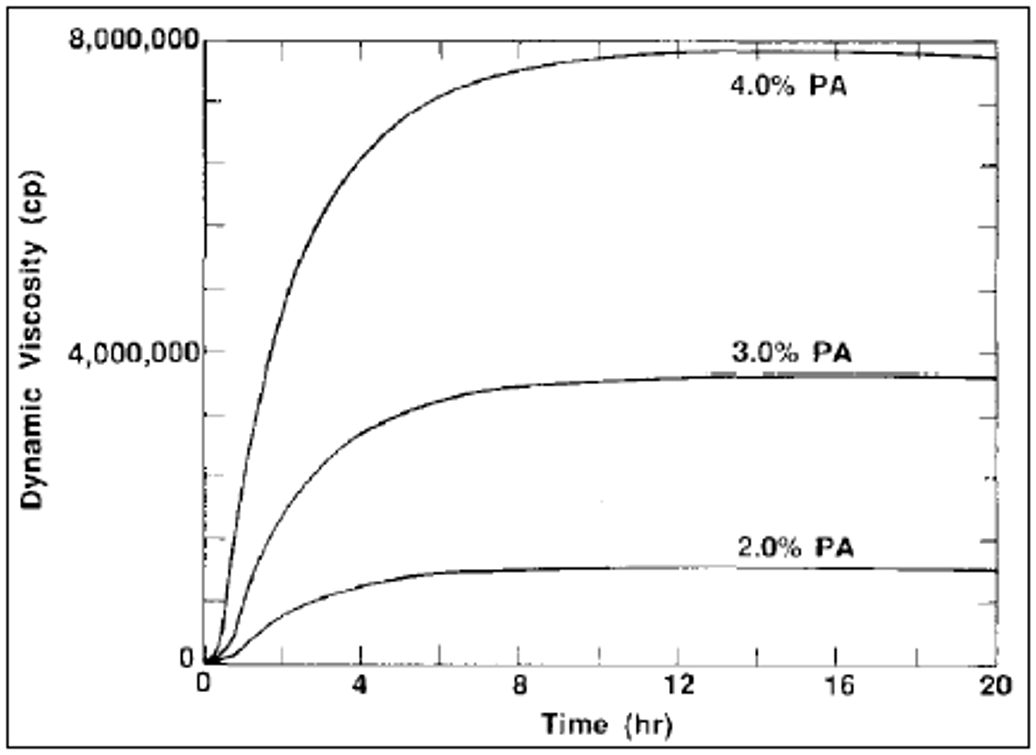
\includegraphics[width=0.75\textwidth]{img/fig/viscSydansk.png}    \caption{Viscosity vs. Time for 2 MDa HPAM (PA) in fresh water aged at 60~\celsius~\citep{Sydansk1993}}
    \label{fig:viscSydansk} % 2.8
\end{figure}

The general findings from the experiments were that as the HPAM concentration increases, the rate of gelation and the dynamic viscosity increase. Other findings include the unchanged rigidity and good stability of the tested gels for more than 730 days.

As has been discussed earlier \citep{Albonico1994}, the increased temperature directly affects the rate of gelation. In order to delay the gelation time, Sydansk concluded from several experiments where low molecular weight polymers (100,000 – 500,000 Da) should be used with ultra-low degree of hydrolysis, $< 0.1$. The phenomenon behind the applicability of using ultra-low hydrolysis degree is auto-hydrolysis that takes place only at elevated reservoir temperatures ($> 75$~\celsius) \citep{Sydansk1993, Fletcher2010}. The rate of auto-hydrolysis is dependent on both temperature and pH.

In order to enhance the thermal stability when HPAM based polymers are considered, other monomers can be co-polymerized with polyacrylamide solutions. Poly(vinylpyrrolidone-co-acrylamide) or PVP-AM is an example of a co-polymerized HPAM base. Polyvinylpyrrolidone improves the PAM base to undergo a lower degree of hydrolysis at elevated temperatures \citep{Stahl1988}. As a result, no precipitation takes place as the conversion of the amide groups into the carboxylate groups is minimized \citep{Al-Muntasheri2012}.

Figure \ref{fig:hyrolysisStahl} shows the degree of hydrolysis at 121~\celsius~ for different PVP-Am (60/40 w/w) and a commercial HPAM. As expected, HPAM-based polymer underwent full hydrolysis in less than 10 days of aging time, and was reported to be insoluble in synthetic seawater \citep{Stahl1988}. PVP-Am experienced a certain degree of hydrolysis and stabilized at 40 \% with no precipitation being reported. Additionally, PVP-AM at 150~\celsius~ did not show signs of precipitation despite reaching 60 \% degree of hydrolysis.

\begin{figure}
    \centering
    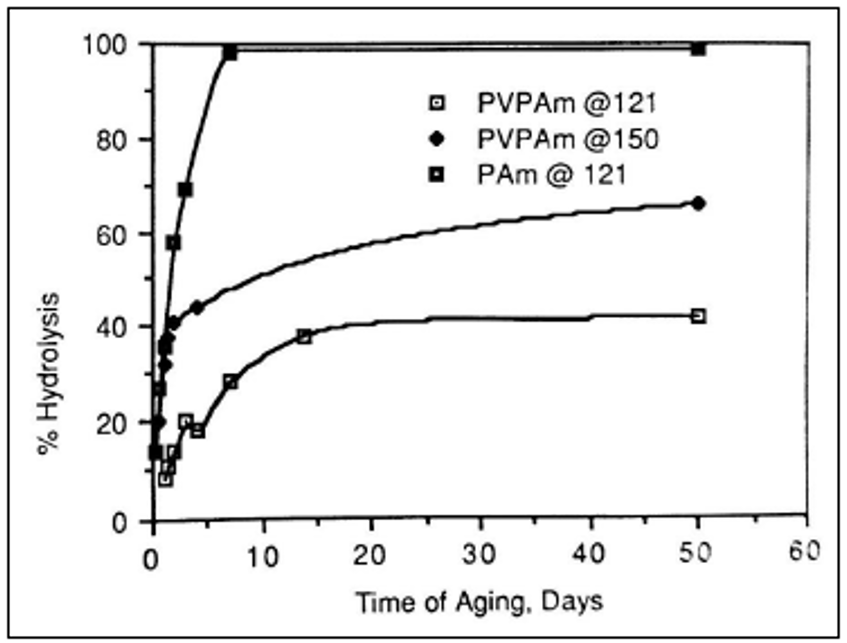
\includegraphics[width=0.75\textwidth]{img/fig/hyrolysisStahl.png}
    \caption{Degree of hydrolysis for different PVP-Am (60/40 w/w) and a commercial HPAM (PAm) \citep{Stahl1988}}
    \label{fig:hyrolysisStahl} % 2.9
\end{figure}

\subsection{Salinity and pH effects}
Gel systems are prepared using different sources of water. Water sources can be considered as either fresh or saline \index{salinity} depending on where it has been obtained from; this can be nearby water wells, treated produced water, or seawater.

\citet{Al-Muntasheri2007} conducted several experiments where two different water sources were examined. Both were used in creating two different gel systems and the apparent viscosity of the polymer solution throughout the gelation period was recorded. The total dissolved solids in the brines were 1186 ppm, and 58348 ppm. Figure \ref{fig:almuntasheriSal} shows the effect of the difference in the salinity of brine. It is clear the effect of increasing the salinity will decrease the gelation time. However, gel systems that were prepared using more saline water exhibited a lower apparent viscosity compared to gel-systems prepared using fresh water.

\begin{figure}
    \centering
    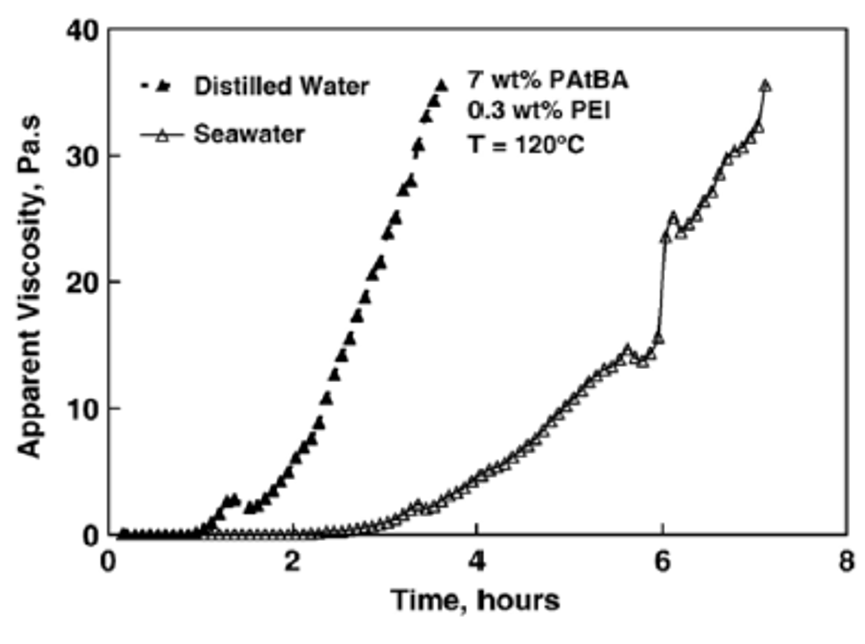
\includegraphics[width=0.75\textwidth]{img/fig/almuntasheriSal.png}
    \caption{Effect of difference in salinity of brine – viscosity vs. time \citep{Al-Muntasheri2007}}
    \label{fig:almuntasheriSal} % 2.10
\end{figure}

In addition, Al-Muntasheri et al. investigated furthermore the possibility that if certain salt ions have a great effect on the gelation compared with others. Monovalent (\ce{K+} and \ce{Na+}) cations were tested as shown in Figure \ref{fig:almuntasheriKNa} which shows that potassium has a greater impact compared with sodium. This has been attributed to the greater charge density which is defined as the ionic charge per size of ion. Similarly, a divalent (\ce{Ca^2+}) cation and monovalent cation (\ce{K+}) were tested as shown in Figure \ref{fig:almuntasheriKCa} and resulted in potassium having a greater impact in extending the gelation time compared with calcium. Again, the same reason is applicable since the charge/size ratio of potassium is only half that of calcium. Therefore, it can be concluded that the gelation time is dependent on the charge/size ratio, rather than the valence of the atom.

\begin{figure}
    \centering
    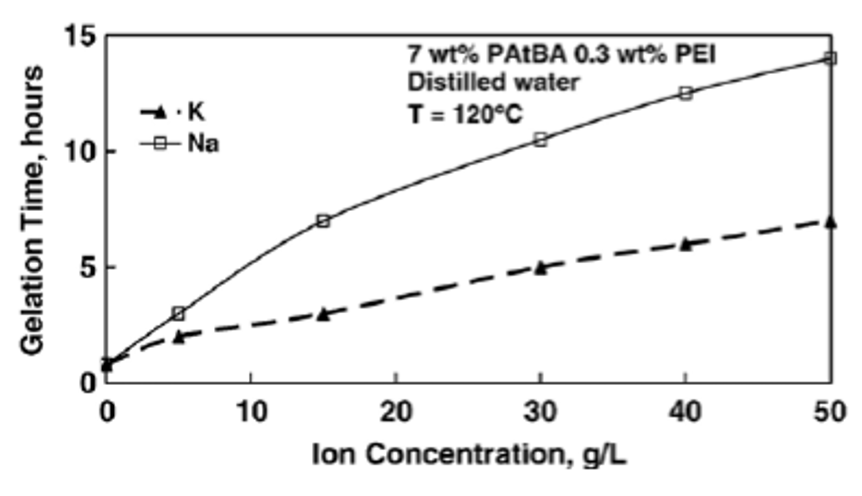
\includegraphics[width=0.75\textwidth]{img/fig/almuntasheriKNa.png}
    \caption{Effect of K and Na cations on gelation time – gelation time vs. ion concentration (PAtBA=A copolymer of acrylamide and tert-butyl acrylate) \citep{Al-Muntasheri2007}}
    \label{fig:almuntasheriKNa} % 2.11
\end{figure}

\begin{figure}
    \centering
    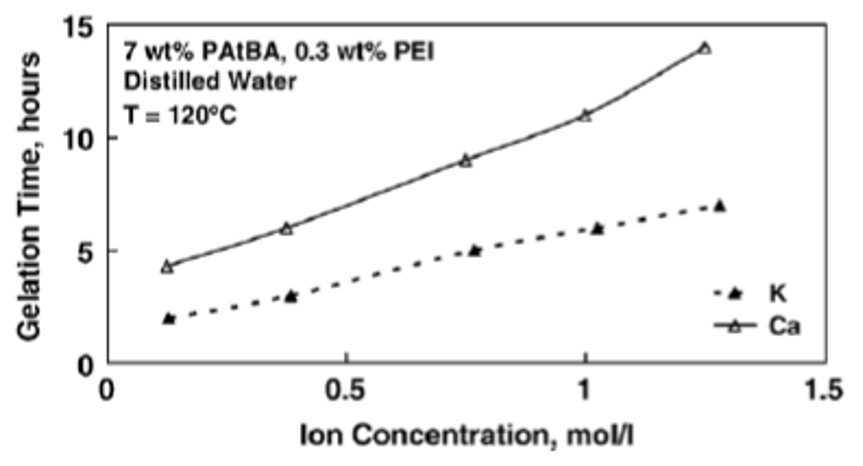
\includegraphics[width=0.75\textwidth]{img/fig/almuntasheriKCa.png}
    \caption{Effect of K and Ca cations on gelation time – gelation time vs. ion concentration \citep{Al-Muntasheri2007}}
    \label{fig:almuntasheriKCa} % 2.12
\end{figure}

The effect of initial \index{pH} pH has been investigated by Al-Muntasheri et al. and the evolution of the viscosity with time was recorded. Adjusting the pH level of the solution could be done by adding variable amount of either HCL (acid) or NaOH (base). Results in Figure \ref{fig:almuntasheriAcidicpH} showed that at very acidic conditions (pH = 3.1) the gel viscosity increased and suddenly collapsed at around 1.3 hours. Furthermore, a less acidic condition (pH = 6.2), a period of stabilization was observed but gel breakage took place at 1.9 hours. 

Following experiments resulted in a conclusion that a basic pH of at least a value of pH = 8 should be considered when designing gel-systems based on PHPA. Figure \ref{fig:almuntasheriBasicpH} shows that the formed gel is stable (opposed to what observed at acidic pH), and the gelation time is dependent on the temperature as discussed in \ref{sec:tempEffects} \citep{Al-Muntasheri2007}.

\begin{figure}
    \centering
    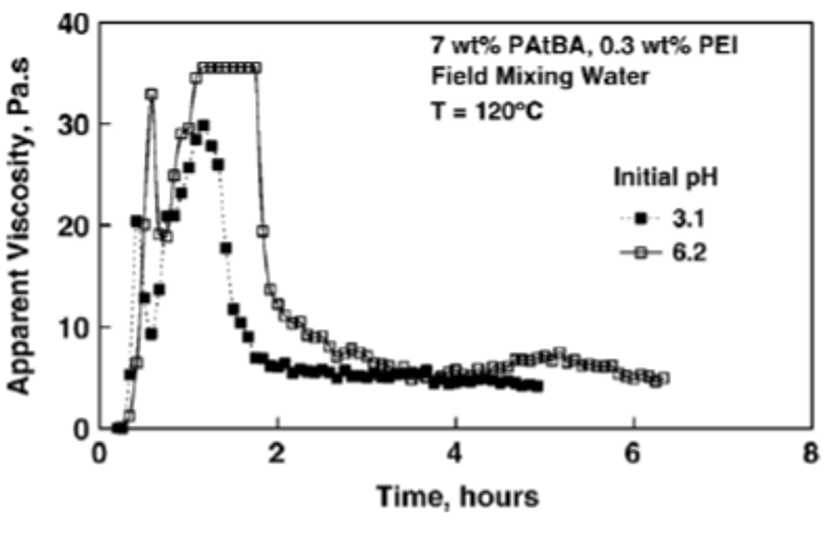
\includegraphics[width=0.75\textwidth]{img/fig/almuntasheriAcidicpH.png}
    \caption{Effect of acidic pH (3.1 and 6.2) at constant temperature – viscosity vs. time \citep{Al-Muntasheri2007}}
    \label{fig:almuntasheriAcidicpH} % 2.13
\end{figure}

\begin{figure}
    \centering
    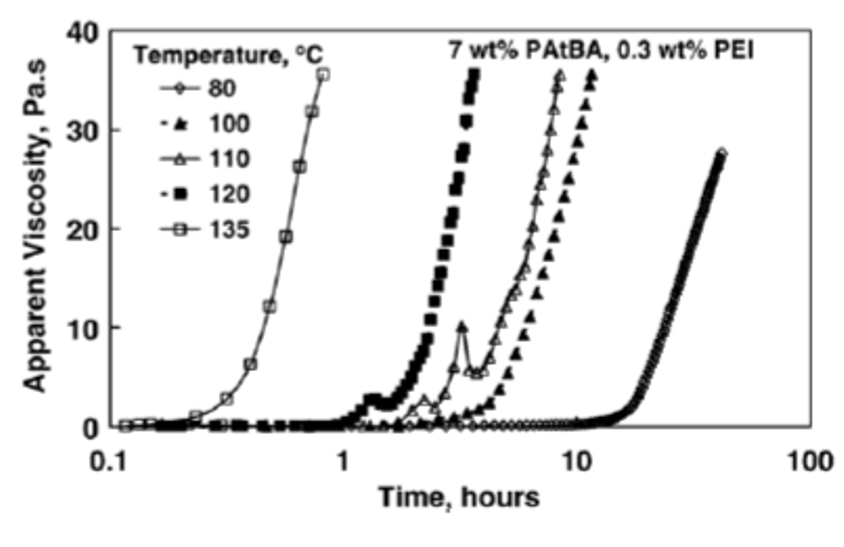
\includegraphics[width=0.75\textwidth]{img/fig/almuntasheriBasicpH.png}
    \caption{Effect of basic pH (8.3) at different temperatures – viscosity vs. time \citep{Al-Muntasheri2007}}
    \label{fig:almuntasheriBasicpH} % 2.14
\end{figure}

\subsection{Hardness effects (concentration of divalent ions)}

HPAM-based polymers have the tendency to precipitate, i.e., they can undergo de-gelation in formations with elevated temperatures with high hardness levels. This is due to the presence of divalent ions, e.g., \ce{Mg^2+}, \ce{Sr^2+}, \ce{Ba^2+}, and \ce{Ca^2+}, where the latter at equal molar levels, has a greater impact on gel stability. Reservoirs with temperatures less than 75~\celsius, the HPAM-based polymers were observed to be stable regardless of the hardness level \citep{Moradi1987}. However, at temperatures higher than 75~\celsius, the amide groups in the polymer experienced extensive hydrolysis, due to the reaction with polyvalent ions present in the formation, which results in weakening the 3D gel network \citep{Al-Muntasheri2012, Stahl1988}. This goes in line with results from experiments reported by \citet{Davison1982} where 140 different HPAM-based polymers were examined at 90~\celsius. Most of them showed precipitation during the several weeks test period.


The situation is more severe when the formation contains higher concentration of hard brines. As the interaction between the amide groups (negative charge) and the divalent cations (positive charge) takes place, precipitation happens in the reservoir causing several negative impacts. Namely, the reduction in mechanical gel strength which leads to the failure of the 3D gel-network, and blockage of the flow in the porous media, leading to a complete shutdown in the injection operations. Carbonate-based gelation retarders can be found in several commercial polymer packages; when they are mixed with water containing high hardness (divalent ions concentration) levels, insoluble carbonate-based salts precipitate in the formation. In case of precipitation, plugging of formation might take place which results in a failure of the water diversion-program, as well as causing injectivity problems leading to a complete shut-down of the operation due to significant pressure increase \citep{Al-Muntasheri2012}.

The results of \citet{Moradi1987} can be taken as a simple reference for brine hardness limits for polyacrylamide-based polymers. Table \ref{tab:formHardnessLim} shows the concentrations of divalent ions in brine after which the gel is no longer stable. For formation brines containing less than 20 ppm, the gels are stable at elevated temperatures of 204~\celsius. This shows the importance of formation hardness of the formation.


\begin{table} 
\centering
\caption{Temperature vs. Formation hardness limit for HPAM \citep{Moradi1987}}
\label{tab:formHardnessLim} % 2.4
\begin{tabular}{c c } 
\toprule
\textbf{Temperature} & \textbf{Formation hardness limit}\\
~[\celsius] & [ppm]\\
\midrule 
75   & 2000\\
88   & 500\\ 
96   & 270\\ 
204   & 20\\ 
\bottomrule
\end{tabular}
\end{table}

Actual precipitation of the gel system (due to hardness levels) is governed by the cloud point temperature. As the temperature of an aqueous solution containing divalent ions is slowly increased, at a certain temperature, the solution will become cloudy; this is referred to as the cloud point. Increasing the temperature to a further extent will lead into precipitation of the gel system. The cloud point can be considered as the upper limit of the temperature at which the gel-system will undergo precipitation, and therefore, all polyacrylamide based polymers design should be based on lower values \citep{Moradi1987, Stahl1988}.

\citet{Moradi1987} conducted several experiments to understand the dependency of the cloud point on \textit{brine hardness level, polymer concentration} and \textit{molecular weight}.

\textbf{Hardness level.} \index{hardness} The cloud point is strongly affected by the hardness level of the brine and the degree of hydrolysis. The temperature at which the cloud point is visible, decreases as both hardness level, and degree of hydrolysis increase. Going from a hardness level of 1 to 10000 ppm (\ce{Ca^2+} + \ce{Mg^2+}), the cloud point dropped from 200~\celsius~ to 170~\celsius~ with 0\% initial degree of hydrolysis, and from 200~\celsius~ to 20~\celsius~ with 93\% degree of hydrolysis.

\textbf{Polymer concentration.} As the polymer concentration increases, the cloud point decreases. It has been shown experimentally that the cloud-point is less affected by the polymer concentration compared with divalent ion concentration. In addition, the cloud time is assumed to be independent at concentrations below 0.25\%, in which most of the applications of polyacrylamides are used at or even below that level in field applications.

\textbf{Molecular weight} seems to influence the cloud point temperature much less compared to the aforementioned investigated parameters. In addition, inconsistent behavior has been obtained from the results when varying the molecular weight. It has been assumed that the reported molecular weights from the vendors might be incorrect.

Determination of the precipitation time, is conducted by plotting the could point temperature versus the hydrolysis level of the selected polymer at different brine hardness levels. As the formation hardness and temperature are usually known, hydrolysis level is the unknown. Next, a plot of hydrolysis level versus time is used to determine the precipitation time of the selected partially hydrolyzed polymer \citep{Moradi1987}.

As discussed earlier, Davison and Mentzer experiments showed that most of the polyacrylamide based polymers precipitated after several weeks. However, polyvinylpyrrolidone is a polyacrylamide based polymer that withstood the temperature at 90~\celsius. Polyvinylpyrrolidone lacks the required viscosity strength for conformance control to be used in IOR operations, however \citep{Stahl1988}.

\section{Environmental considerations} \label{sec:environmental}
Injection of chemicals, \index{environment} i.e. polymers in case of in-depth water diversion applications, imposes certain risks related to environmental concerns. In the petroleum industry, chemicals are usually classified by colour codes based on their eco-toxicity. In Norway, four colour codes were suggested by "Klima- og forurensingsdirektoratet" (Klif), an Norwegian directorate that is responsible for regulating the chemical discharge permits. Figure \ref{fig:envColors} shows the definitions of each colour code \citep{Norskolje2018}.

\begin{figure}
    \centering
    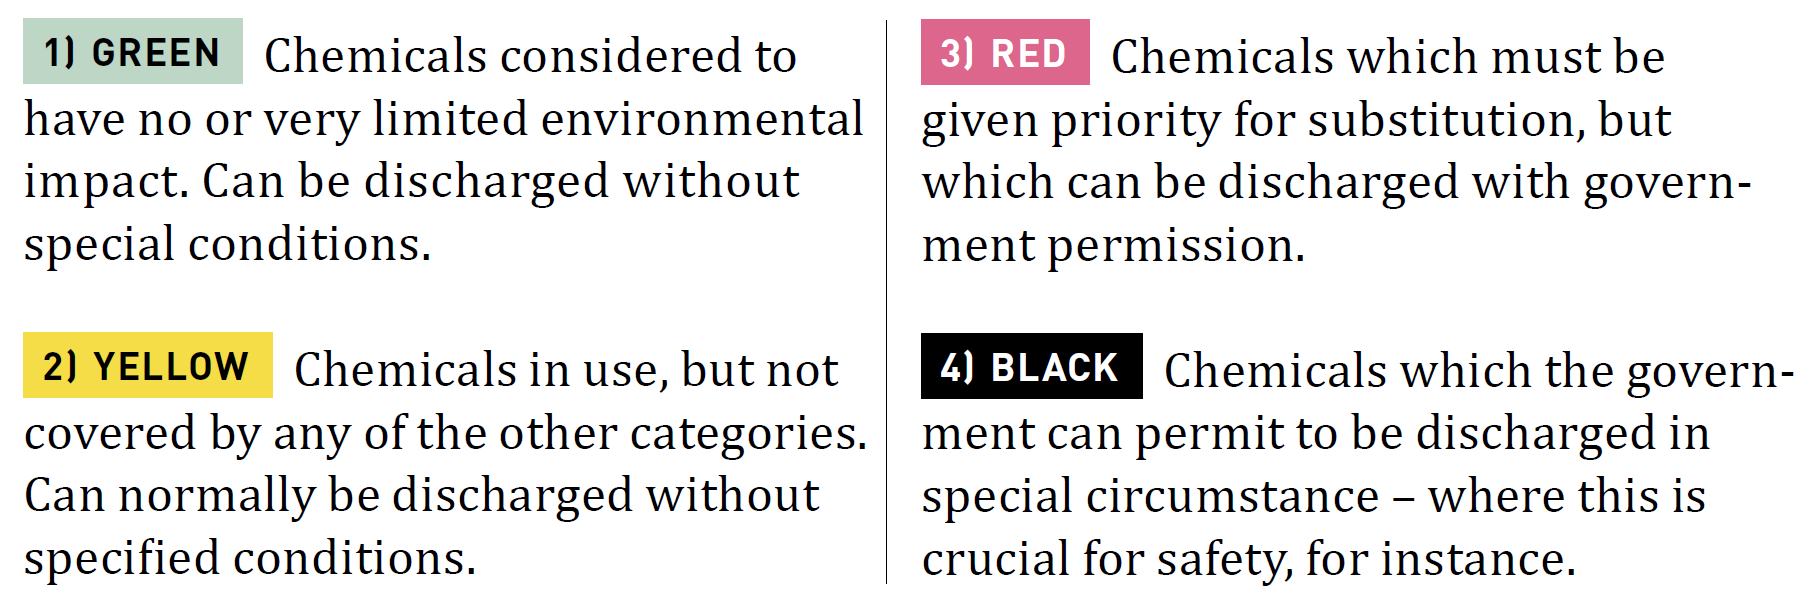
\includegraphics[width=\textwidth]{img/fig/envColors.png}
    \caption{Toxicity color definitions based on Klif classification \citep{Norskolje2018}}
    \label{fig:envColors} % 2.15
\end{figure}

The use of the red and black chemicals on the Norwegian Continental Shelf (NCS) has declined in the past years clearly as stricter laws were enforced and substituents were considered. Figure \ref{fig:colorsNcs} shows an extreme decline in year 2003 for red and black coded chemicals. Discharges of chemical additives from Norwegian petroleum operations in 2016 contained 90.6\% green, 9.4\% yellow, 0.07\% red, and 0.002\% black chemicals \citep{Norskolje2018}. 

\begin{figure}
    \centering
    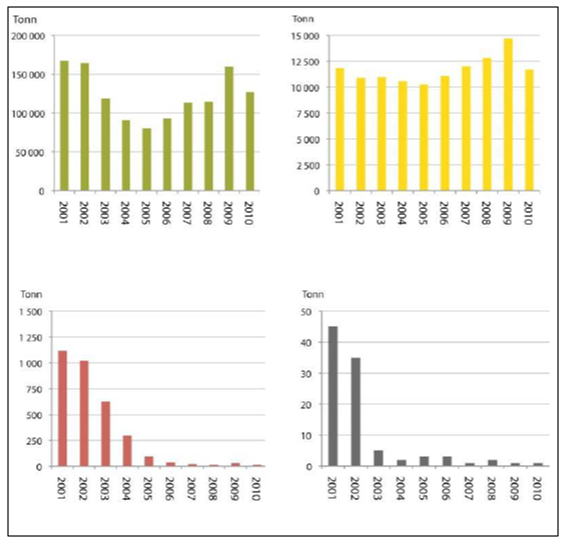
\includegraphics[width=\textwidth]{img/fig/colorsNcs.png}
    \caption{Green, yellow, red and black chemicals discharge in NCS  \citep{Norskolje2018}}
    \label{fig:colorsNcs} % 2.16
\end{figure}

Chemicals that are planned to be injected in the NCS reservoirs for EOR purposes have to be tested for eco-toxicological properties. Namely, these tests are: biodegradability, bioaccumulation, and acute toxicity \citep{Force2012}.

Biodegradability can be defined as the biological breakdown of materials by microorganisms, e.g. bacteria, fungi and algae \citep{Leja2010}. Bioaccumulation refers to the phenomenon where chemicals are accumulated in fish due to feeding on other species, usually smaller fish in size, that contain these chemicals in their bodies \citep{Beek2000}. That is, top fish predators that are highest in the food chain, like Cod, will contain the highest amount of persistent chemicals \citep{Koster2001}. 

Persistent chemicals refer to the type of chemicals that do not break down over time and will remain in the body of the fish; this includes mercury, polychlorinated biphenyls (PCB), dichlorodiphenyl trichloroethane (DDT), dioxins, and hexachlorocyclohexan (HCB) \citep{Adedipe2010}. Acute toxicity, or acute effects, is the harmful effects that happen to mammals after a first contact or exposure to a source of contamination, i.e. a chemical that is used for IOR purposes in the scope of this paper \citep{Cheremisinoff1996}.

The Norwegian regulations imply zero-discharge policy. However, according to Klif, the use of red classified chemicals does not contradict the statement when the produced water is re-injected, and not discharged. In addition, gel systems that are designed to remain in the reservoir for in-depth water diversion are not in contradiction with the zero-discharge policy, even if the colour classification is red such as “Bright water” chemicals that have been used in Heidrun field in-depth water diversion operations \citep{Am2010} [in the Bright water approach a suspension of crosslinked polymers are injected, which go through hydrolysis triggered by temperature, and swell up as a result.]

In 2008, Statoil ASA, Norske Shell, and Total E\&P Norge initiated a research project entitled “Environmental Aspects of EOR Chemicals – Phase I” for addressing environmental challenges associated with the use of HPAM for EOR applications on the Norwegian continental shelf \citep{Force2012}. The project was conducted at SINTEF and was completed within 3 years, highlighting several important findings and recommendations. 

For water-conformance applications using gel systems, the gel is designed to remain in the formation for as long as possible. However, in case of unsuccessful operations where no gelation occurs, or cases where the gel system becomes unstable, i.e. undergoing precipitation or breakage after some time, it is possible that these gel fragments are produced \citep{Force2012}.

The appropriate environmental solution to deal with this produced water or PFPW (Polymer-flooding produced water) is to consider produced water re-injection and limit discharging the produced water into the sea, which is illegal according to Norway’s regulations. However, these regulations approve the discharge of produced water after treatment. The current challenge is that there does not exist an efficient technology for treating HPAM \citep{Azrague2011}. Therefore, there is a need to understand the properties and behaviour of the selected gel system in the operation.

Furthermore, it has been found that HPAM, which is classified as a red chemical, has low degradation, i.e. for 28 days less than 20\% of the HPAM is degraded. As an attempt to reduce the environmental impact of HPAM, and comply with the Norwegian offshore discharge laws, several forced degradation methods were considered to make the use of HPAM environmentally acceptable \citep{Azrague2011}. 

The SINTEF research group found that hydrolysis, oxidation, UV irradiation, ultrasound and thermal degradation demand much energy and the degradation process which is relatively slow. In addition, mechanical degradation was found to be faster but demands even more energy. Eventually, it has been concluded that the method of advanced oxidation processes was efficient and the most compact degradation solution and therefore suitable for offshore operations due to space limitations \citep{Azrague2011}.

Further findings from the research group highlight the existence of several methods to detect and monitor HPAM concentrations offshore that give rough estimates. However, lab studies should be conducted for accurate characterization. The research group concluded by recommending that the best approach to deal with the back-produced water is to treat it first using cost effective methods, and then re-inject it. In case of discharging the back-produced water to the sea, the aforementioned degradation methods should be considered so that the HPAM will be biodegraded faster by marine species \citep{Azrague2011}.

\subsection{Environmental effects of crosslinkers}

 The organic cross-linkers \index{cross-linker} in Section \ref{sec:PolyacrylamideGels} showed robust results at withstanding high-temperatures for extended periods of time due to the strong covalent bond. However, these organic cross-linkers, e.g. formaldehyde and phenol-based polymers, are not environmentally friendly. Replacement of these chemical components with less toxic products is often considered. For instance, formaldehyde is substituted by hexamethylenetetramine, glyoxal, paraformaldehyde, acetaldehyde, propionaldehyde and butyraldehyde. Furthermore, phenol can be replaced by other components such as hydroquinone, resorcinol, pyrogallol, and phenyl salicylate \citep{SinghYadav2013}.

The most applied metal cross-linkers in polymer-based gel systems are \ce{Al^3+}, \ce{Zr^4+}, \ce{Cr^3+}. In the United States of America, \ce{Cr^3+}  is not considered toxic but it is regulated \citep{AgencyforToxicSubstancesandDiseaseRegistry2012}. However, \ce{Cr^3+} is classified as a red chemical in Norway. It is important to note that \ce{Cr^6+} can also be applied as a crosslinking with the advantage of delaying the gelation time. But due to its proven toxicity and carcinogenic attributes, its use in gel systems is no longer allowed \citep{Al-Muntasheri2012}. Aluminum (\ce{Al^3+}) exists naturally in reservoir rocks and therefore it is much safer than \ce{Cr^3+}. Gel systems crosslinked with \ce{Al^3+} can be applied only in reservoir conditions with low temperature and pH \citep{Xin2013, Osman2013}.

A holistic evaluation should be conducted to determine the environmental impact due to the use of the selected gel system and cross-linkers, and the possible solutions that can be applied in case of operational failures.
